\documentclass[letter,graphicx]{beamer}



\mode<presentation>
{
  \usetheme{Warsaw}
  % or ...

  \setbeamercovered{transparent}
  % or whatever (possibly just delete it)
}


\usepackage[english]{babel}
% or whatever

\usepackage[latin1]{inputenc}
% or whatever
\usepackage{verbatim}
\usepackage{times}
\usepackage[T1]{fontenc}
\usepackage{mychicago}
\renewcommand{\citeN}{\shortciteN}
% Or whatever. Note that the encoding and the font should match. If T1
% does not look nice, try deleting the line with the fontenc.

\logo{\includegraphics[width=.1\textwidth]{./images/official_NOAA_logo.pdf}}

\title[microhaplotypes from NGS] % (optional, use only with long paper titles)
{Reaching haplotopia: the promise and practice \\
of short-read microhaplotypes\\
in molecular ecology}

\subtitle{} % (optional)

\author[Eric C. Anderson] % (optional, use only with lots of authors)
{Eric C.~Anderson and the NMFS-SWFSC-MEGA Team}
% - Use the \inst{?} command only if the authors have different
%   affiliation.

\institute[NOAA Fisheries] % (optional, but mostly needed)
{\mbox{}
%Fisheries Ecology Division \\ Southwest Fisheries Science Center \\ Santa Cruz, CA \\ USA
\hfill
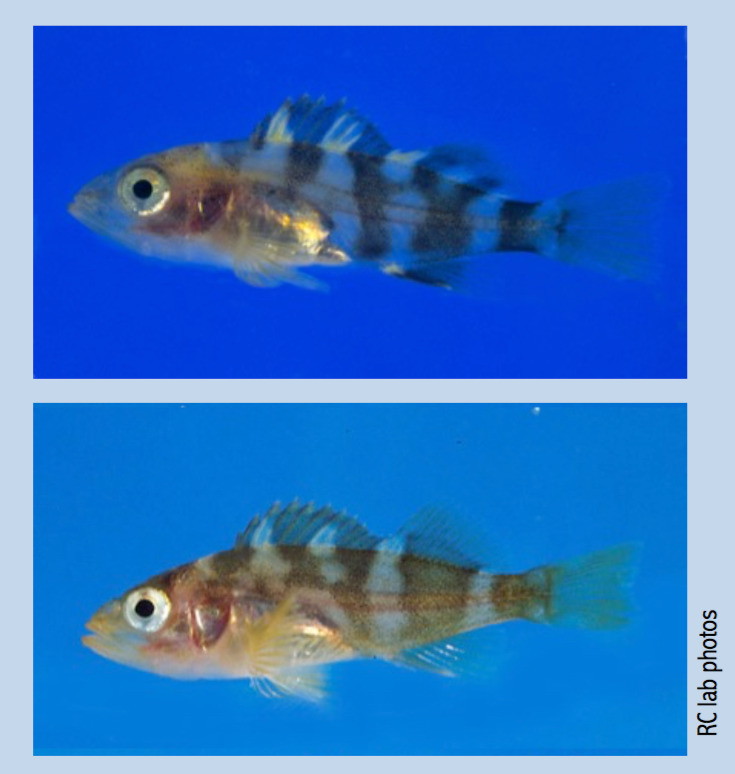
\includegraphics[height=.25\textwidth]{./mhap_figs/juvie_rockfish.png}
\hfill
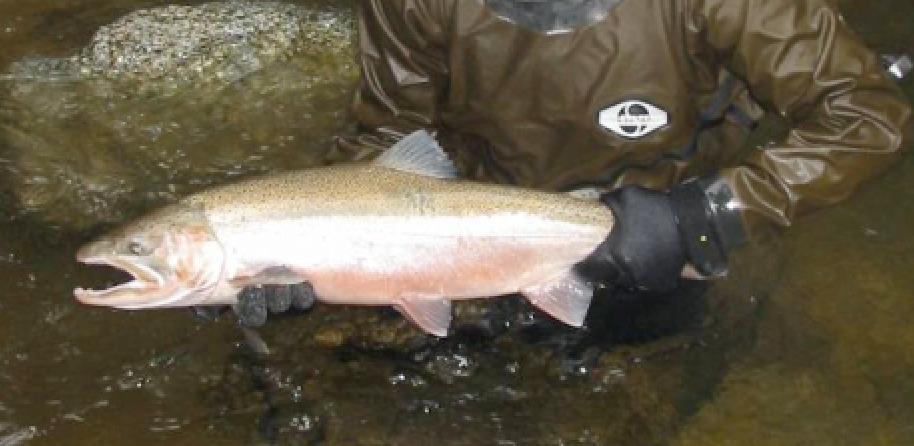
\includegraphics[height=.25\textwidth]{./mhap_figs/steelhead.png}
\hfill\mbox{}
}
% - Use the \inst command only if there are several affiliations.
% - Keep it simple, no one is interested in your street address.

\date[Durham 2016] % (optional)
{
Durham University Ecology Seminar\\ 14 NOV 2016}

\subject{Talks}


%% More eric commands for inserting some small figures
\newcommand{\smikid}{\includegraphics[width=3.7ex]{images/smiley_blue_kid.pdf}}
\newcommand{\smired}{\includegraphics[width=2.9ex]{images/smiley_sad_red.png}}
\newcommand{\smiblue}{\includegraphics[width=2.9ex]{images/smiley_happy_blue.png}}
\newcommand{\thh}{^\mathrm{th}}
\newcommand{\tc}{\textcolor}
\def\bm#1{\mathpalette\bmstyle{#1}}
\def\bmstyle#1#2{\mbox{\boldmath$#1#2$}}


\begin{document}




\begin{frame}
  \titlepage
\end{frame}



%	Chris Edwards <cedwards@ucsc.edu>,
%Mark Carr <mhcarr@ucsc.edu>,
%John Carlos Garza <carlos.garza@noaa.gov>,
%"Eric C. Anderson" <eric.anderson@noaa.gov>,
%Emily Saarman <esaarman@ucsc.edu>,
%Daniel Malone <dmalone@ucsc.edu>,
%Patrick Drake <pdrake@ucsc.edu>,
%Anna Lowe <ablowe@ucsc.edu>
% Thomas Ng
% Diana Baetscher
%


\begin{frame}{Overview}
\begin{itemize}
\item Next Generation Sequencing Methods
\begin{itemize}
\item sequencing, assembly, alignment
\item genome representation reduction
\item amplicon sequencing
\end{itemize}

\item Microhaplotypes
\begin{itemize}
\item available by reanalysis of most data sets
\item advantages
\end{itemize}

\item Example problem: Dispersal of larval rockfish
\begin{itemize}
\item parentage and sibling inference in a multispecies context
\end{itemize}

\item Tools from our lab:
\begin{itemize}
\item CKMRsim
\item haPLOType
\end{itemize}

\end{itemize}
\end{frame}







\begin{frame}{Next Generation Sequencing -- I}
\framesubtitle{Illumina Sequencing By Synthesis}
{\centering
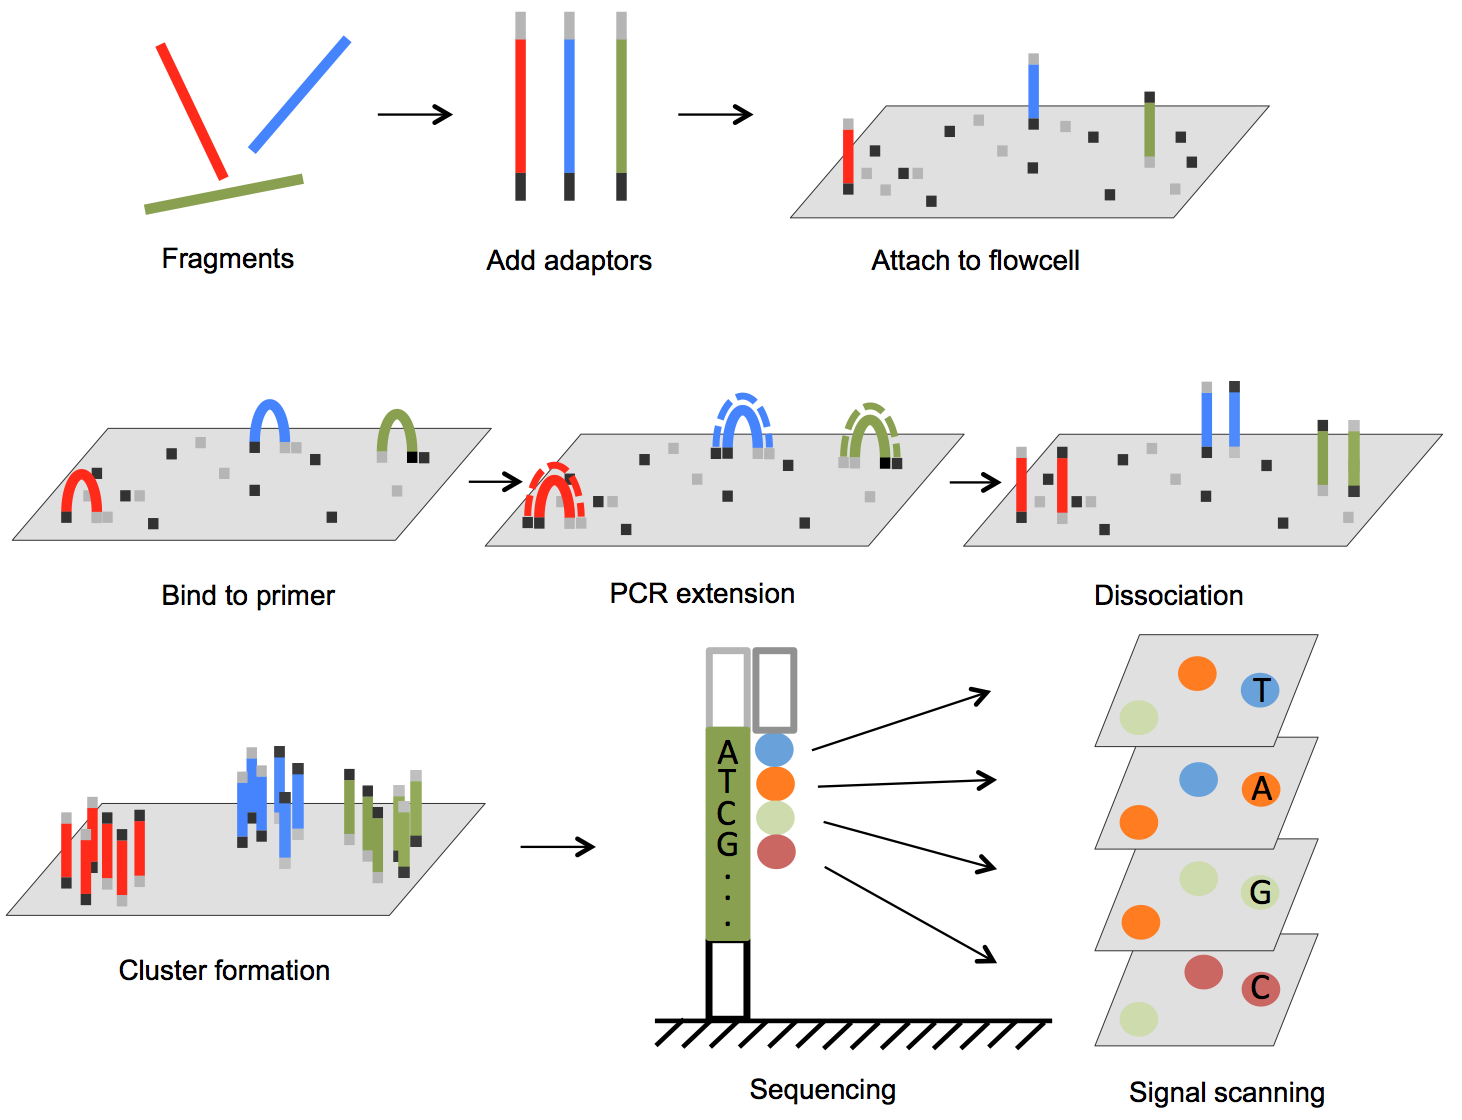
\includegraphics[height=0.80\textheight]{mhap_figs/illumina_fig.png}
}\\
{\tiny http://www.intechopen.com}
\end{frame}







\begin{frame}{Next Generation Sequencing -- II}
\framesubtitle{{\em de novo} ``genome'' assembly}
{\centering
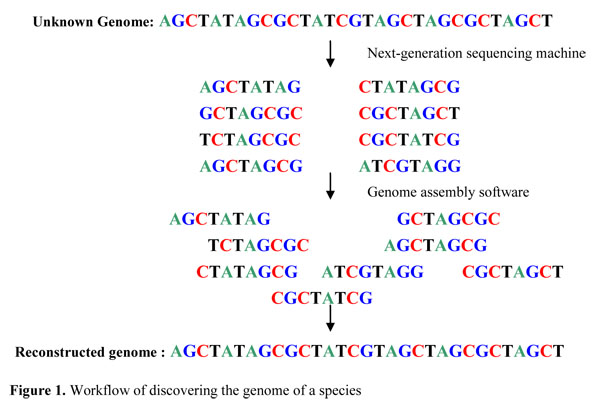
\includegraphics[height=0.75\textheight]{mhap_figs/assembly.png}
}\\
{\tiny http://www.cs.hku.hk}
\end{frame}






\begin{frame}{Next Generation Sequencing -- III}
\framesubtitle{Alignment of sequencing reads to ``genome'' allows \\
identification of polymorphisms and genotyping}
{\centering
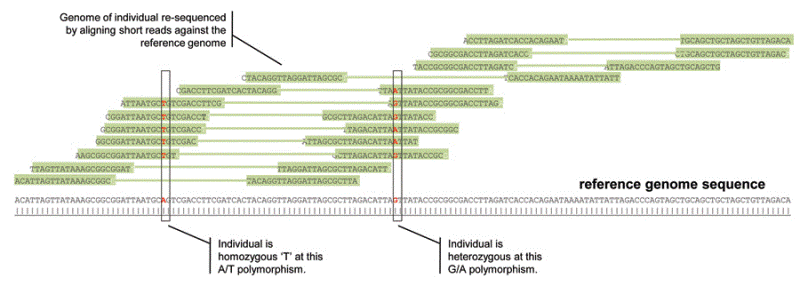
\includegraphics[width=0.95\textwidth]{mhap_figs/alignment.png}
}\\
{\tiny http://www.historyofnimr.org.uk}
\end{frame}






\begin{frame}{Sequencing Capacities}
\framesubtitle{Continually increasing.  Examples from Illumina:}
\begin{itemize}
\item Small Benchtop MiSeq sequencer:
\begin{itemize}
\item 25 million reads/run ($\approx \$1,000$ reagent cost)
\item up to 2 x 300 bp
\end{itemize}

\item Large Core facility HiSeq sequencer:
\begin{itemize}
\item 500 million reads per lane ($\approx \$3,400$)
\item up to 2 x 150 bp
\end{itemize}
\end{itemize}


\begin{itemize}
\item {\em Many} individuals can be sequenced together via combinatorial barcoding.
\end{itemize}
\end{frame}





\begin{frame}{Combinatorial Barcodes}
$\bullet$ Imagine that you prepared individuals in batches (plates) of three at time.\\
$\bullet$ Individual barcode on one end; plate barcode on the other.
\begin{center}
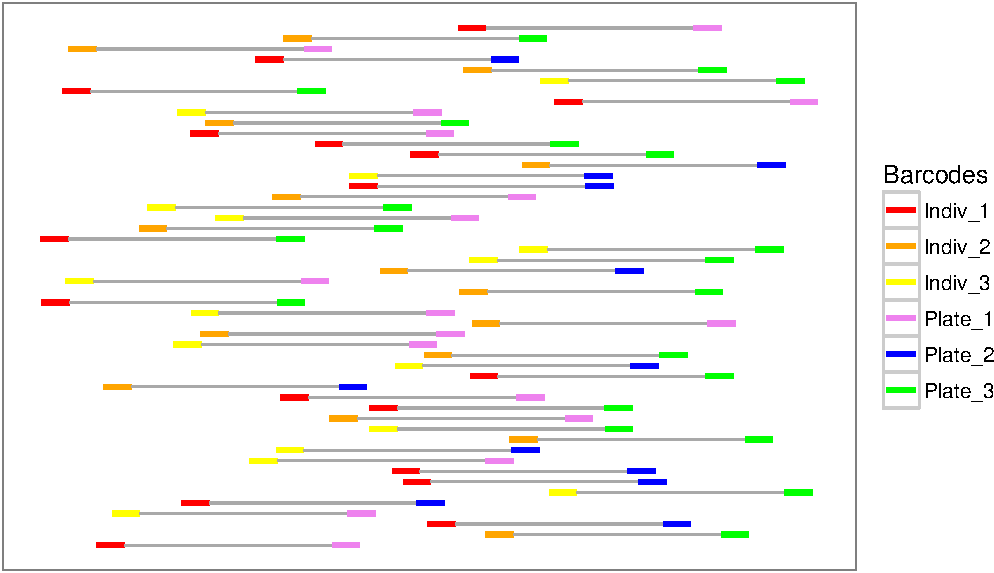
\includegraphics[width=.95\textwidth]{mhap_figs/combi-barcodes-crop.pdf}
\end{center}
\end{frame}






\begin{frame}{Fundamental Tradeoff}
\begin{itemize}
\item Accurate determination of the sequence {\em at a genomic position} and {\em in an individual} requires a sufficient number of reads sequencing that position in that individual.
\item So, either:
\begin{itemize}
\item One (or a few) individuals across large swaths of genome
\item Many individuals across a reduced portion of the genome
\end{itemize}
\item Methods for {\em reduced representation} sequencing:
\begin{itemize}
\item RNAseq (sequence just the transcriptome)
\item RADseq (Restriction Associated DNA sequencing)
\item GBS (Genotyping by Sequencing)
\item Capture/Bait methods (MyBaits, RAPTURE, etc.)
\item Amplicon Sequencing (GTseq)
\end{itemize}
\end{itemize}
\end{frame}





\begin{frame}{GTseq amplicon sequencing}
\begin{center}
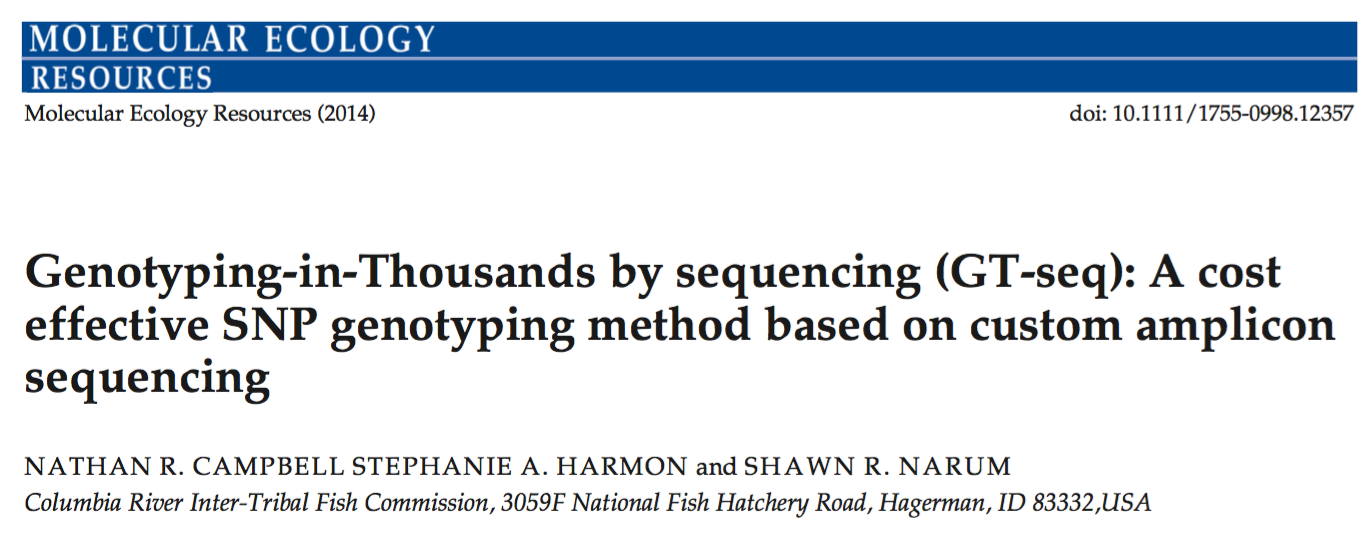
\includegraphics[width=0.95\textwidth]{mhap_figs/gtseq-header.png}
\end{center}
\begin{itemize}
\item Multiplexed PCR primers amplify regions of interest.
\item Amplicon sequencing of 200--500 regions in 500--2,000 individuals
\item $\approx \$7$/individual
\item Converted Fluidigm SNP assays.  Tens of 1,000s of salmon each year.
\end{itemize}
\end{frame}








\begin{frame}{GTseq -- I {\small (coming off the sequencer\ldots)}}
\framesubtitle{2 Amplicons; 3 individuals on each of 3 plates (9 individuals total)}
\begin{center}
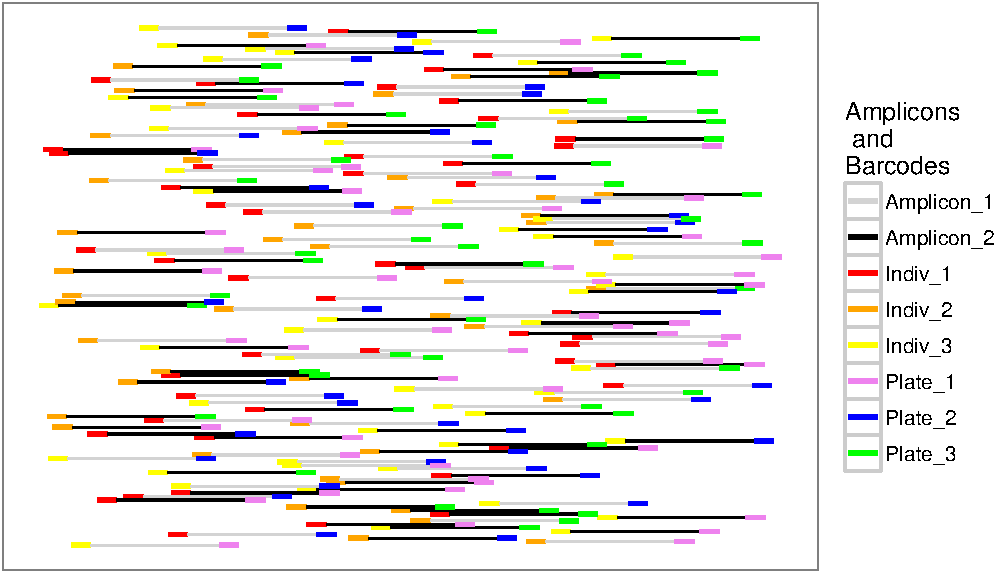
\includegraphics[width=0.95\textwidth]{mhap_figs/gtseq-soup-crop.pdf}
\end{center}
\end{frame}





\begin{frame}{GTseq -- II (aligned amplicons)}
\framesubtitle{Amplicon sequences are known. Alignment {\em in silico} is straightforward.}
\begin{center}
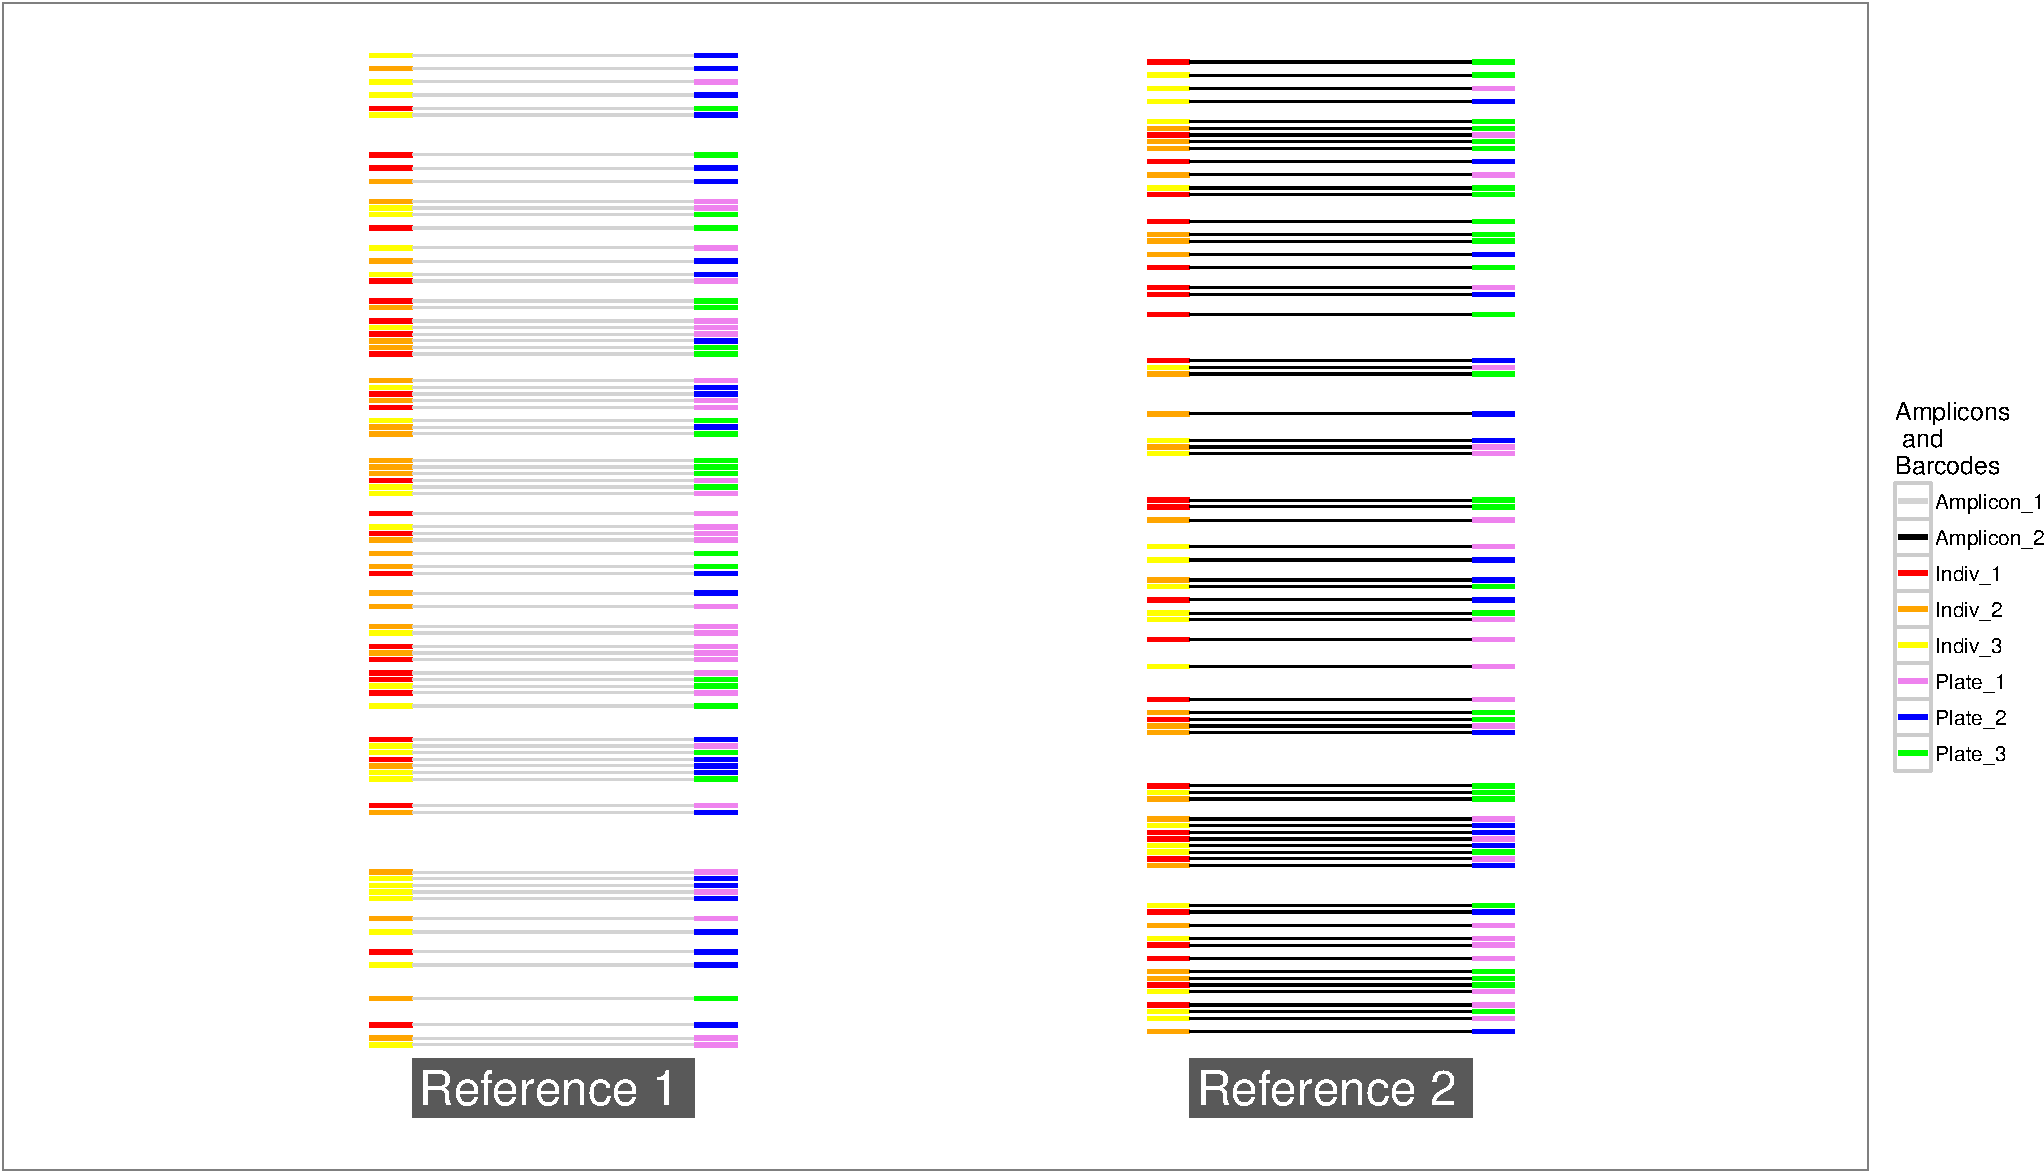
\includegraphics[width=0.95\textwidth]{mhap_figs/gtseq-amps-crop.pdf}
\end{center}
\end{frame}



\begin{frame}{GTseq -- III (``demultiplexing'')}
\framesubtitle{Identify individual origin of reads via combinatorial barcodes}
\begin{center}
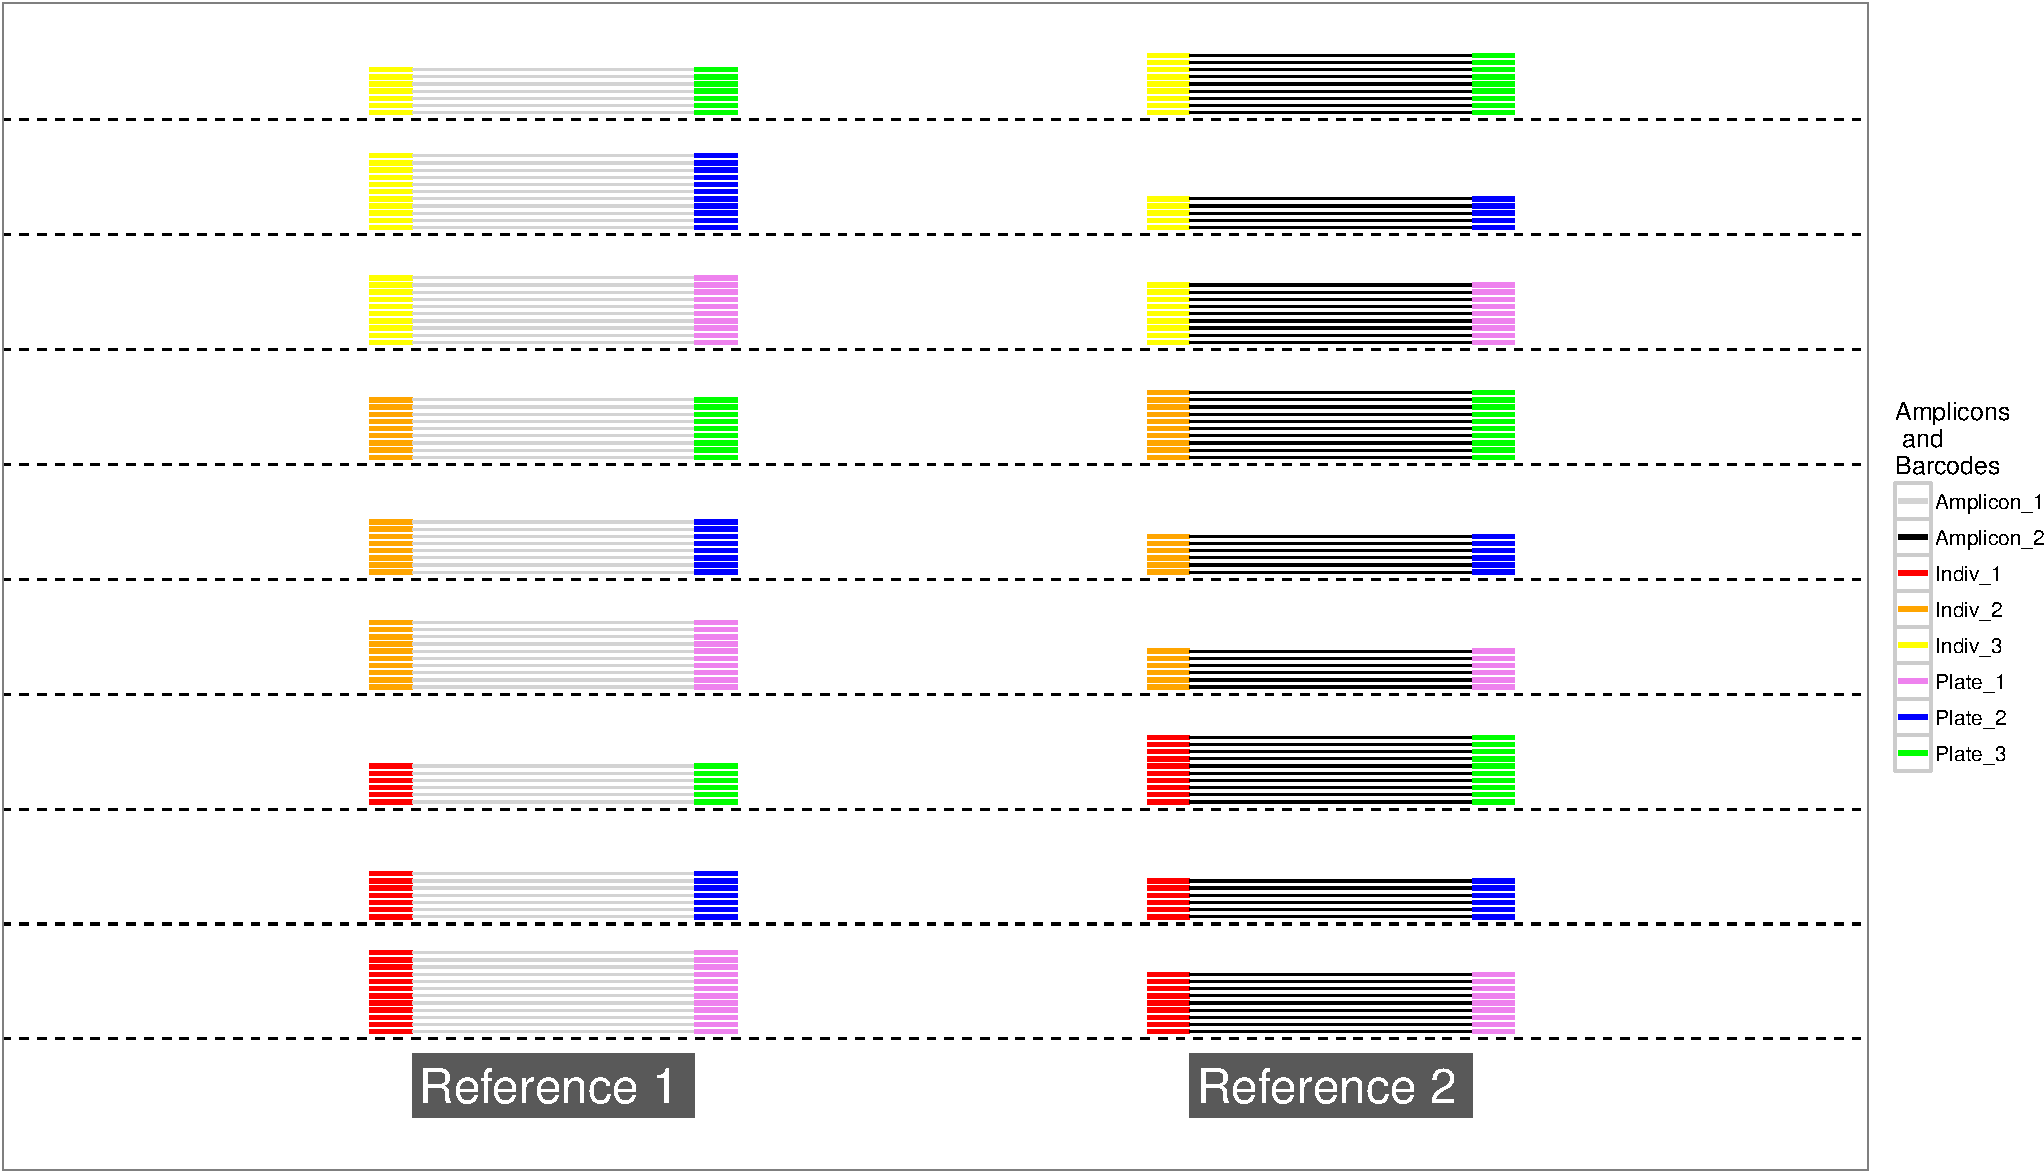
\includegraphics[width=0.95\textwidth]{mhap_figs/gtseq-demultiplexed-crop.pdf}
\end{center}
\end{frame}





\begin{frame}{GTseq -- IV (identify SNPs in sequence)}
\framesubtitle{Variants are easy to identify}
\begin{center}
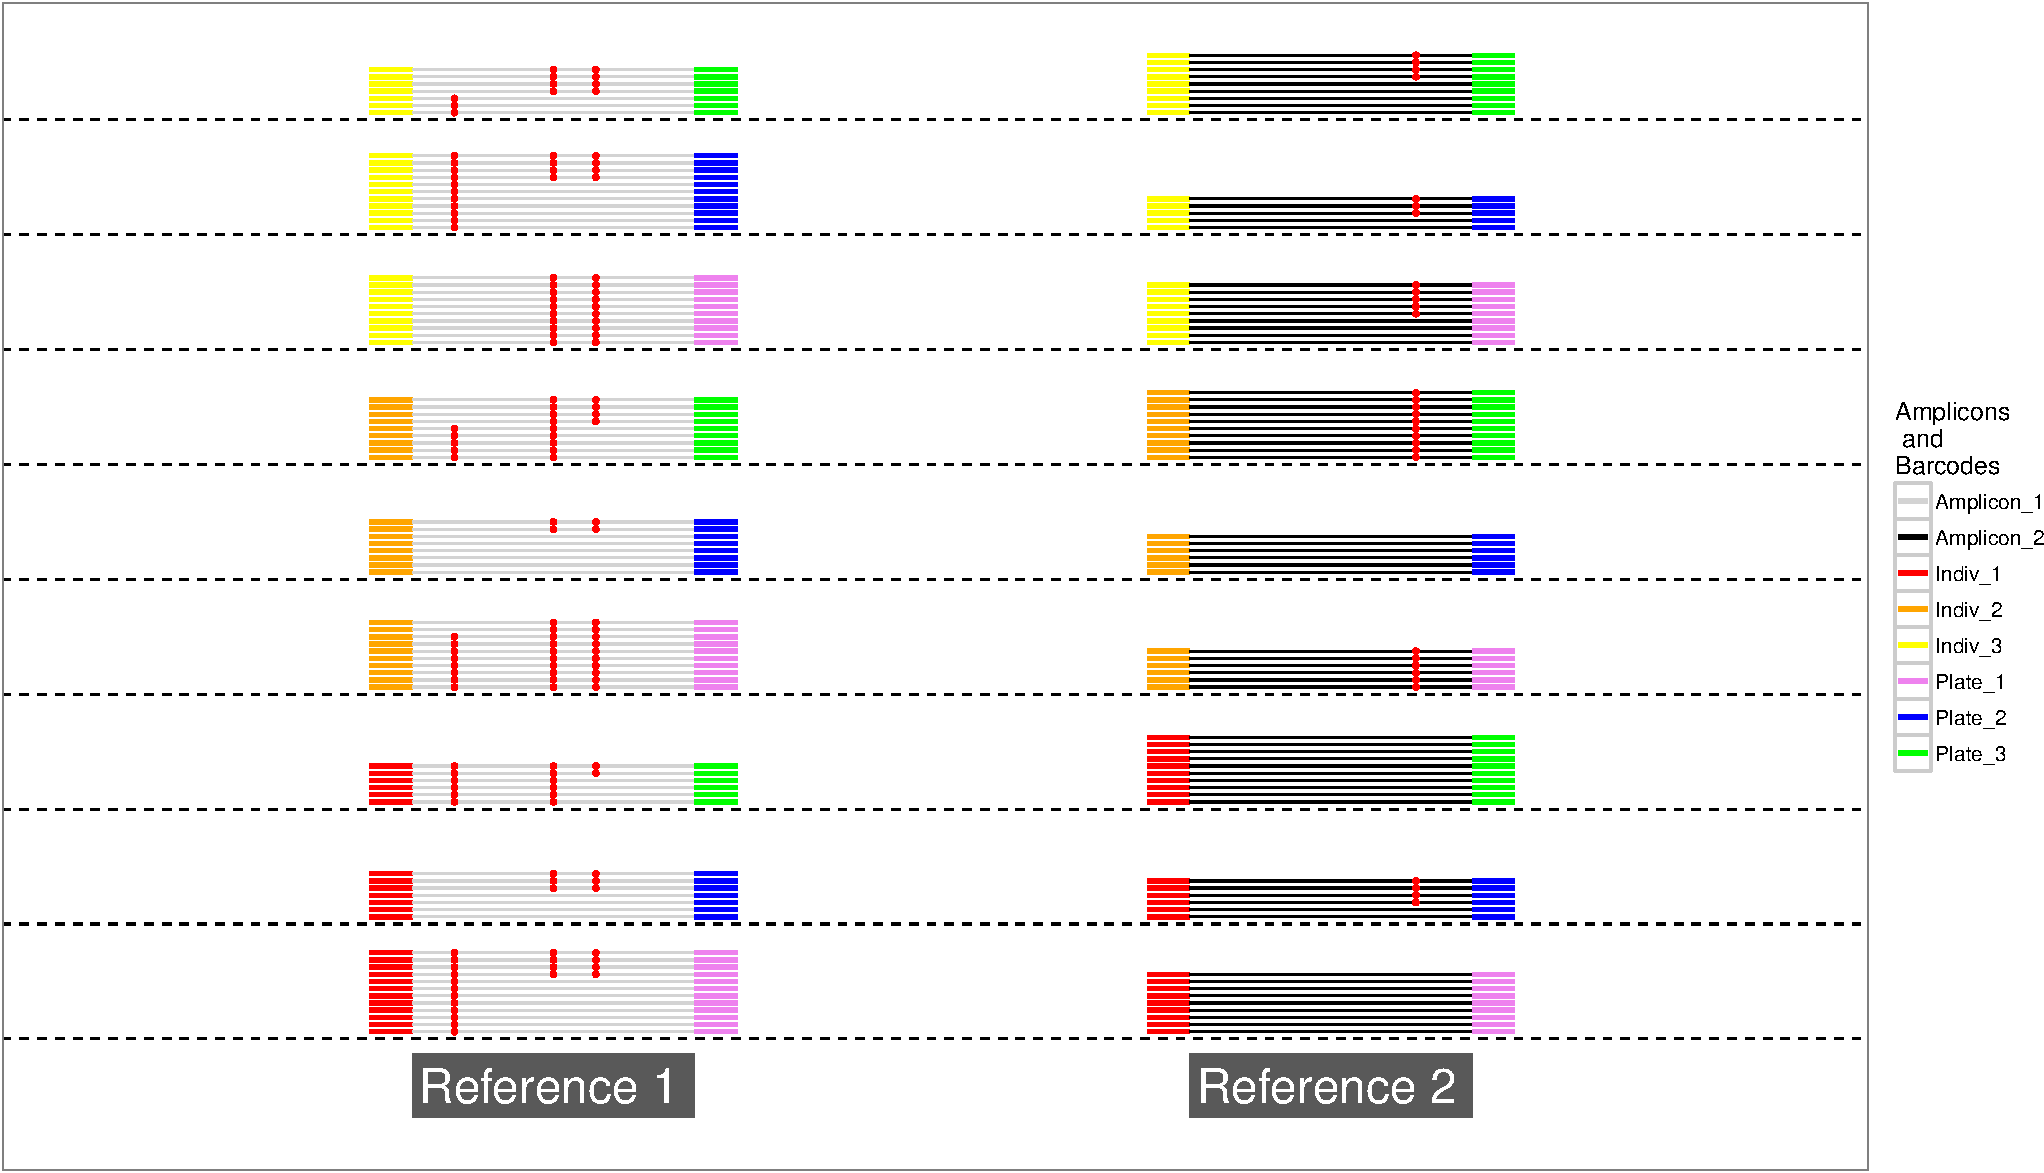
\includegraphics[width=0.95\textwidth]{mhap_figs/gtseq-snps-crop.pdf}
\end{center}
\end{frame}




\begin{frame}{Multiple SNPs in amplicons/sequences\ldots}
\framesubtitle{\ldots are almost universally ignored }
\begin{itemize}
\item Multiple SNPs in each amplicon/RAD-locus are typically scored
\item But then either:
\begin{enumerate}
\item Only a single SNP from each amplicon/locus is used
\item OR, all SNPs are treated as unlinked
\end{enumerate}
Depending on the analyses, the result is either a lack of power or (potentially) incorrect inference.
\end{itemize}
\end{frame}






\begin{frame}{Phase of SNPs on reads is almost universally ignored}
\begin{center}
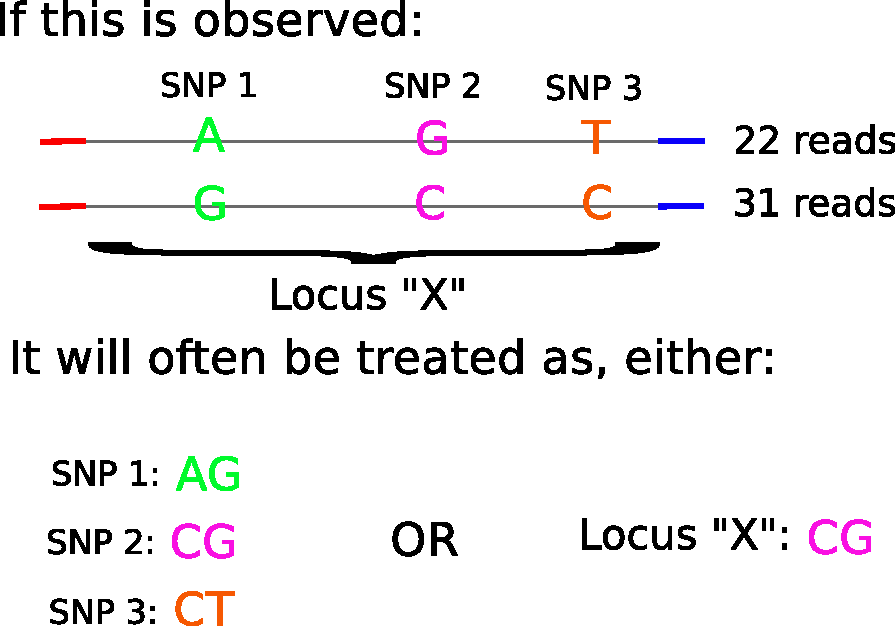
\includegraphics[width=0.94\textwidth]{mhap_figs/three-snp-reads.pdf}
\end{center}
\end{frame}













\begin{frame}{Microhaplotypes}
\framesubtitle{A simple idea / plea, that\ldots}
\begin{center}
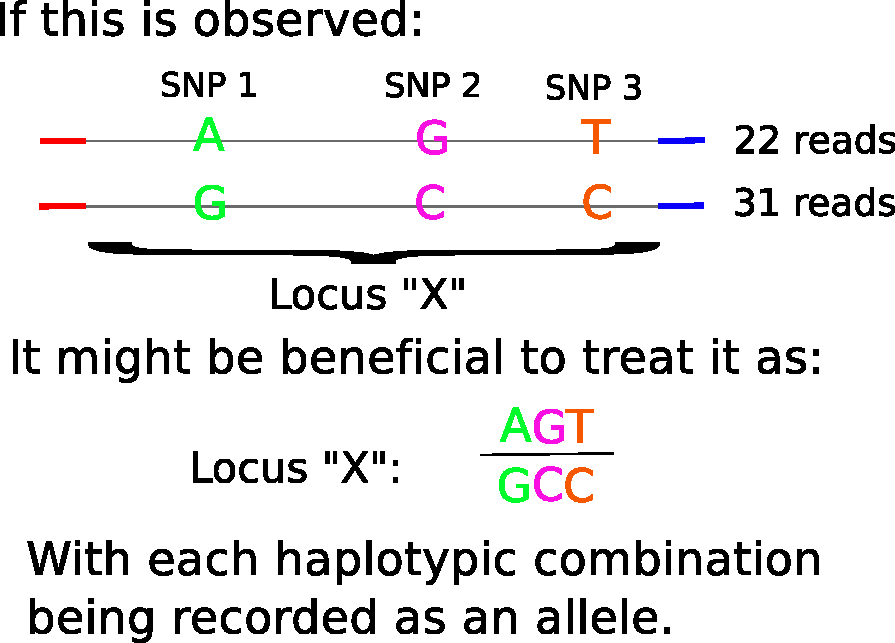
\includegraphics[width=0.94\textwidth]{mhap_figs/three-snp-reads-mhap.pdf}
\end{center}
\end{frame}






\begin{frame}{Microhaplotypes}
\framesubtitle{Potential advantages}
\begin{itemize}
\item Multiallelic loci
\begin{itemize}
\item More power for relationship inference / pedigree reconstruction
\end{itemize}
\item Need not discard SNPs from certain loci
\begin{itemize}
\item Retain low-frequency variants.  Useful for population structure in recently diverged populations.
\end{itemize}
\item Amplicons typically cross-amplify between closely-related species
\begin{itemize}
\item Unlike single SNP assays, the microhaplotype data collection method, unmodified,
can yield useful data for non-target species.
\end{itemize}
\end{itemize}
\end{frame}







\begin{frame}{Marine Population Structure}
\begin{columns}
\begin{column}{0.45\textwidth}
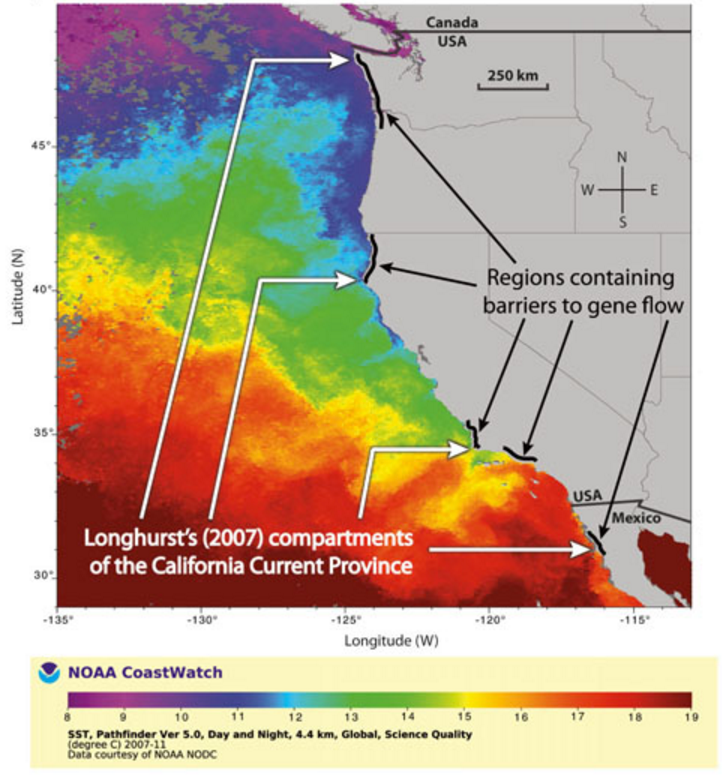
\includegraphics[width=1.1\textwidth]{mhap_figs/vetter_coast.png}\\
{\tiny Hyde and Vetter (2009) CJFAS}
\end{column}
\begin{column}{0.55\textwidth}  %%<--- here
\begin{itemize}
\item California Current
\begin{itemize}
\item Upwelling; nutrients; long larval duration
\end{itemize}
\item Barriers to gene flow
\begin{itemize}
\item Suspected from patterns of genetic variation
\item Difficult to estimate actual migration/dispersal rates
\end{itemize}
\item Considerable interest in larval dispersal/retention
\begin{itemize}
\item Design of MPAs, etc.
\end{itemize}
\end{itemize}

\end{column}
\end{columns}
\end{frame}




\begin{frame}{Larval Dispersal off California}
\framesubtitle{Heavily influenced by Ekman transport}
\begin{columns}
\begin{column}{0.45\textwidth}
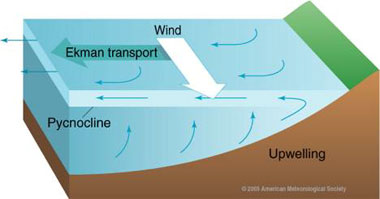
\includegraphics[width=\textwidth]{mhap_figs/ekman-upwelling.jpg}\\
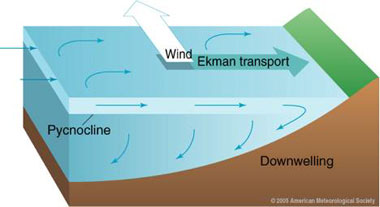
\includegraphics[width=\textwidth]{mhap_figs/ekman-downwelling.jpg}\\
{\tiny Amer. Meterol. Soc.}
\end{column}
\begin{column}{0.55\textwidth}  %%<--- here
\begin{itemize}
\item Typical Pattern:
\begin{itemize}
\item Winds blowing south down coast
\item Water transport offshore
\end{itemize}
\item Periods of relaxation:
\begin{itemize}
\item Winds blowing to the north
\item Water transport toward shore
\end{itemize}
\item Larval recruit origins
\begin{itemize}
\item Coarse current models suggest most come from far away
\item BUT, Fine-scale current irregularities might allow local
larval retention 
\end{itemize}

\end{itemize}

\end{column}
\end{columns}


\end{frame}








\begin{frame}{Question:}
\framesubtitle{What is the degree of larval self-recruitment around Carmel Bay?}
\begin{columns}
\begin{column}{0.45\textwidth}
\mbox{}\hspace*{-1ex}
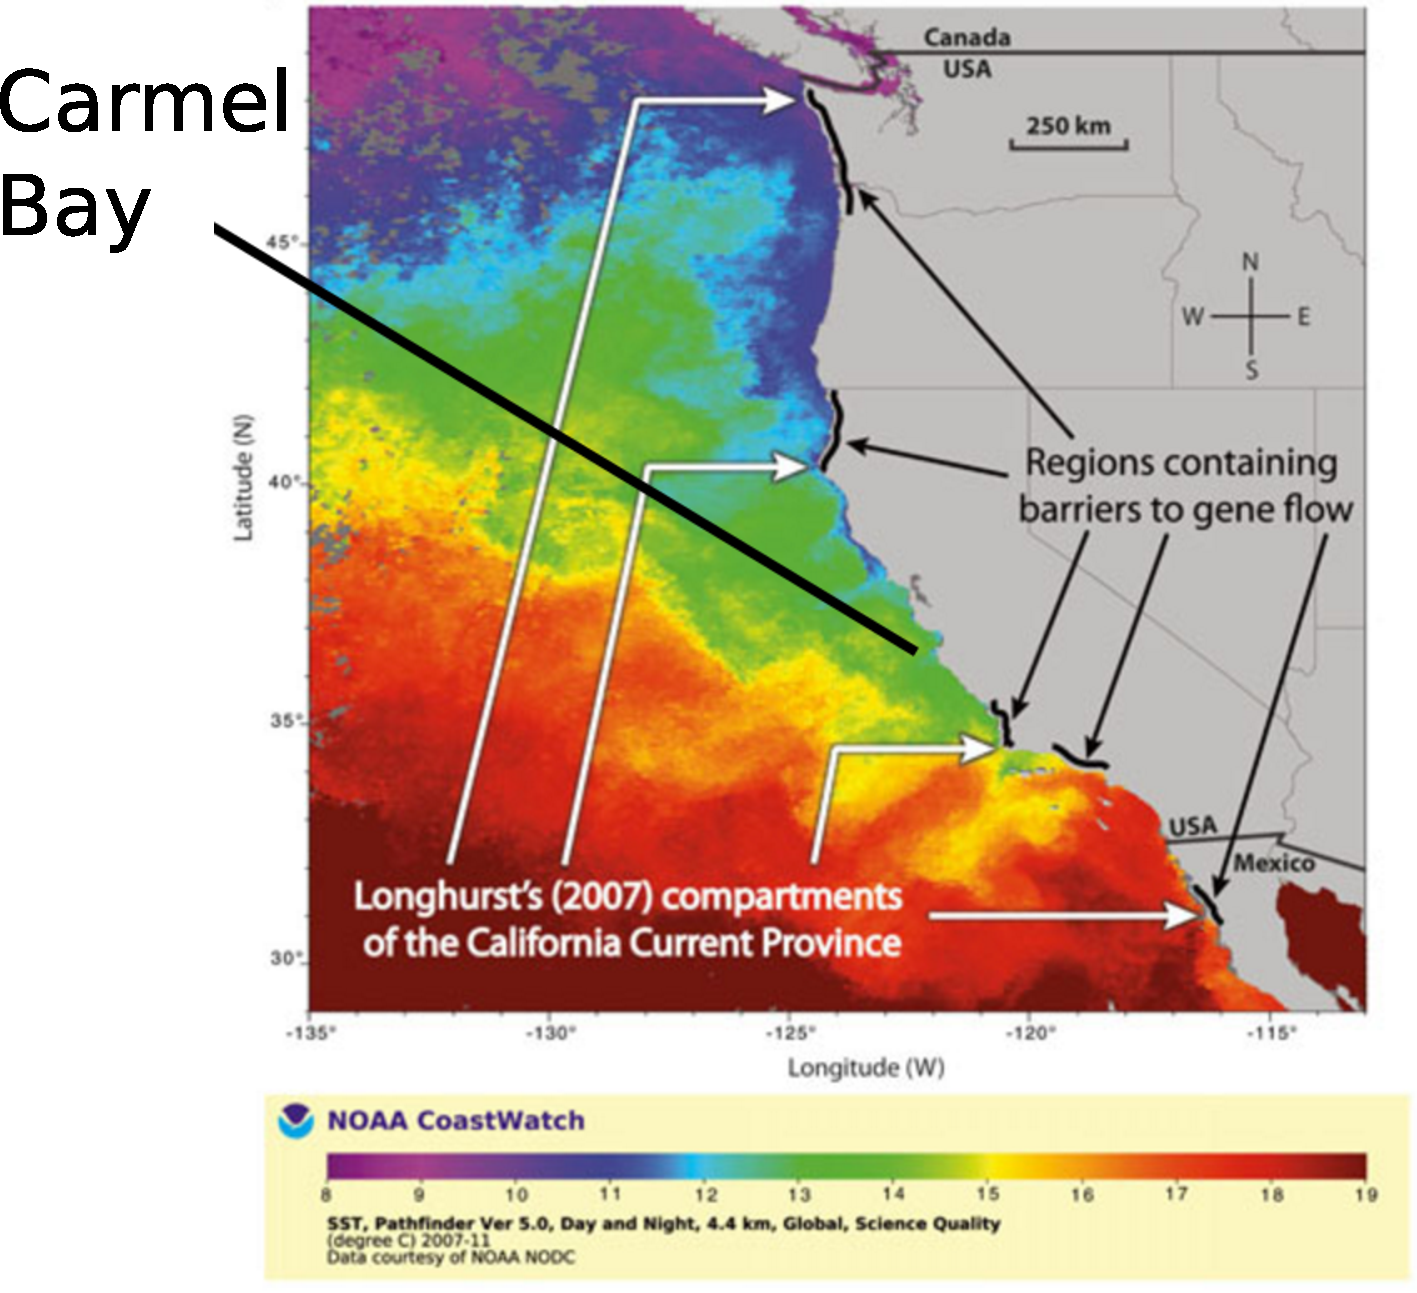
\includegraphics[width=1.2\textwidth]{mhap_figs/vetter_coast-CB.pdf}\\
{\tiny Hyde and Vetter (2009) CJFAS}
\end{column}
\begin{column}{0.55\textwidth}  %%<--- here
\begin{itemize}
\item Experimental Approach with Kelp Rockfish
\begin{enumerate}
\item Non-lethally sample a boatload ($\approx 5,000$) of adult fish
\item Genotype them
\item Collect tissues from $\approx 5,000$ larval recruits
\item Genotype them
\item Find parent-offspring pairs
\end{enumerate}
\end{itemize}
\end{column}
\end{columns}
\end{frame}











\begin{frame}{Kelp Rockfish ({\em Sebastes atrovirens})}

{\tiny photo: Wikimedia}
\includegraphics[width=0.9\textwidth]{mhap_figs/Sebastes_atrovirens.jpg}\\
Adults stationary.  Sampled by biopsy spear or hook-and-line.  Very active volunteer 
``recreational-sampling'' component. 
\end{frame}




\begin{frame}{SMURF traps}
\framesubtitle{Standard Monitoring Unit for the Recruitment of Reef Fishes}
\begin{center}
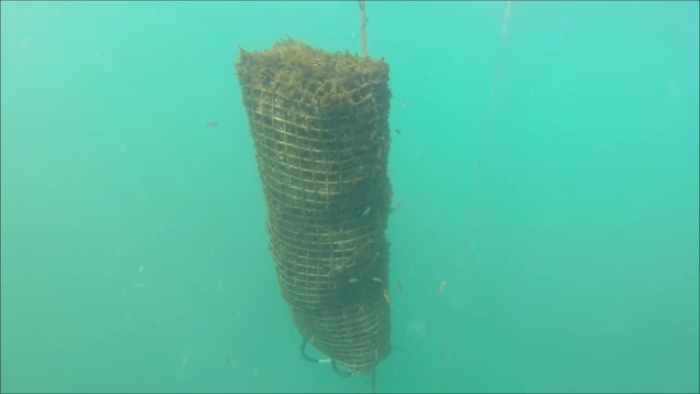
\includegraphics[width = 0.85\textwidth]{mhap_figs/smurf-solo.png}\\
{\tiny Carr-Raimondi lab photo}
\end{center}
\end{frame}



\begin{frame}{SMURF traps}
\framesubtitle{Standardized protocol for juvenile collection}
\begin{center}
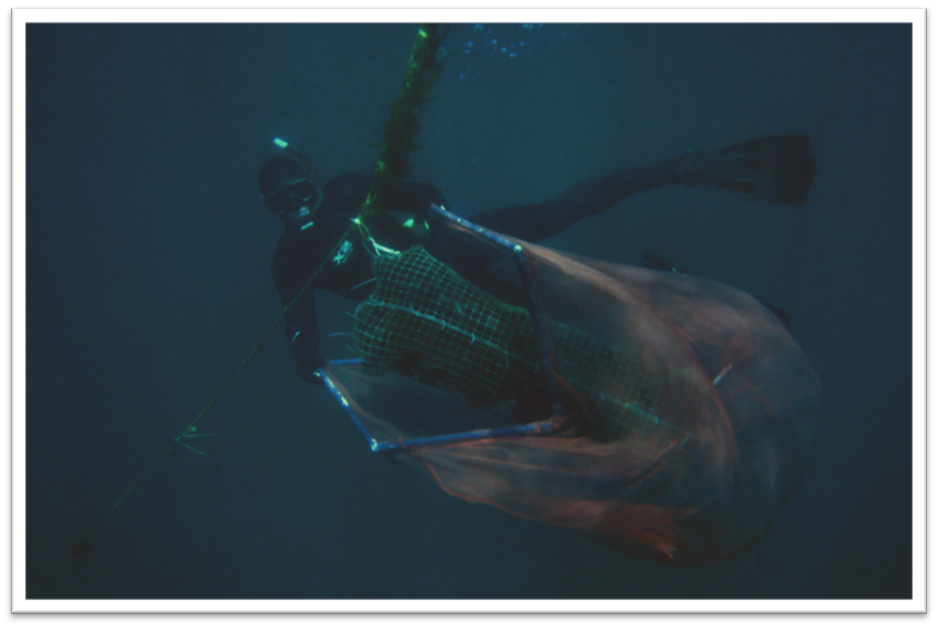
\includegraphics[width = 0.85\textwidth]{mhap_figs/smurf-binkie.png}\\
{\tiny Carr-Raimondi lab photo}
\end{center}
\end{frame}





\begin{frame}{Originally-proposed approach}
\framesubtitle{Large-scale parentage inference with microfluidic SNP assays}
\begin{center}
\mbox{}\hspace*{-.10\textwidth}
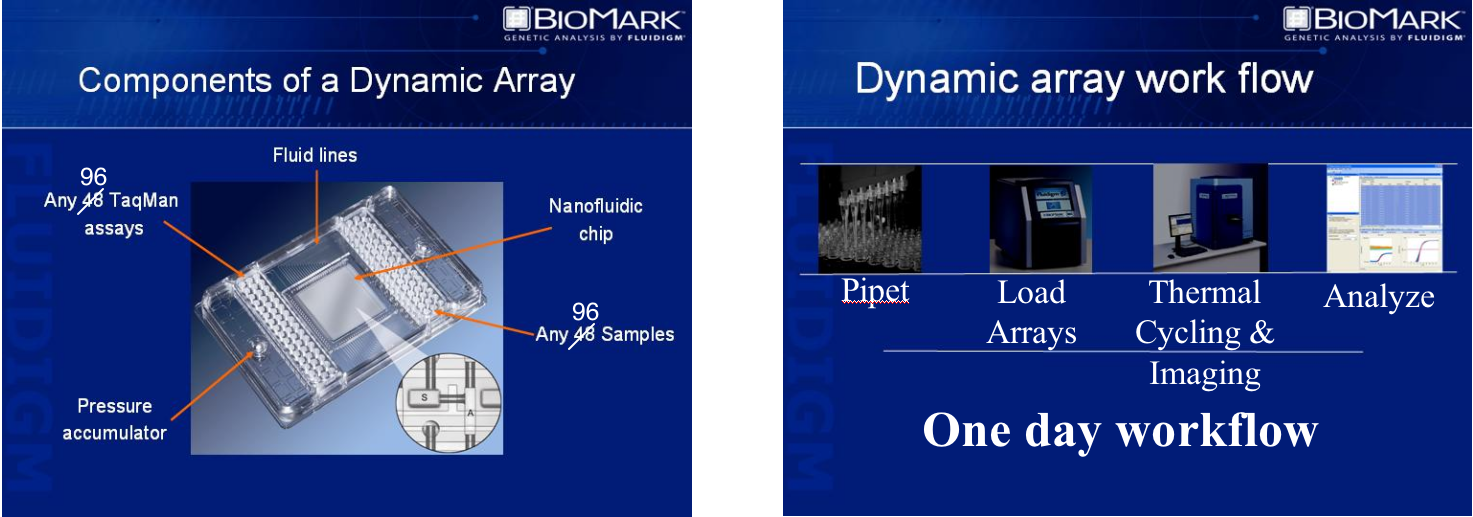
\includegraphics[width=1.16\textwidth]{mhap_figs/fluidigm.png}\\
With 96.96 Arrays and only one controller and thermal cycler, \\
can genotype almost 300 fish per day w/96 SNPs.

Cost: $<$\$15/fish 
\end{center}
\end{frame}








\begin{frame}{Nanofluidic chips, a known quantity}
\begin{center}
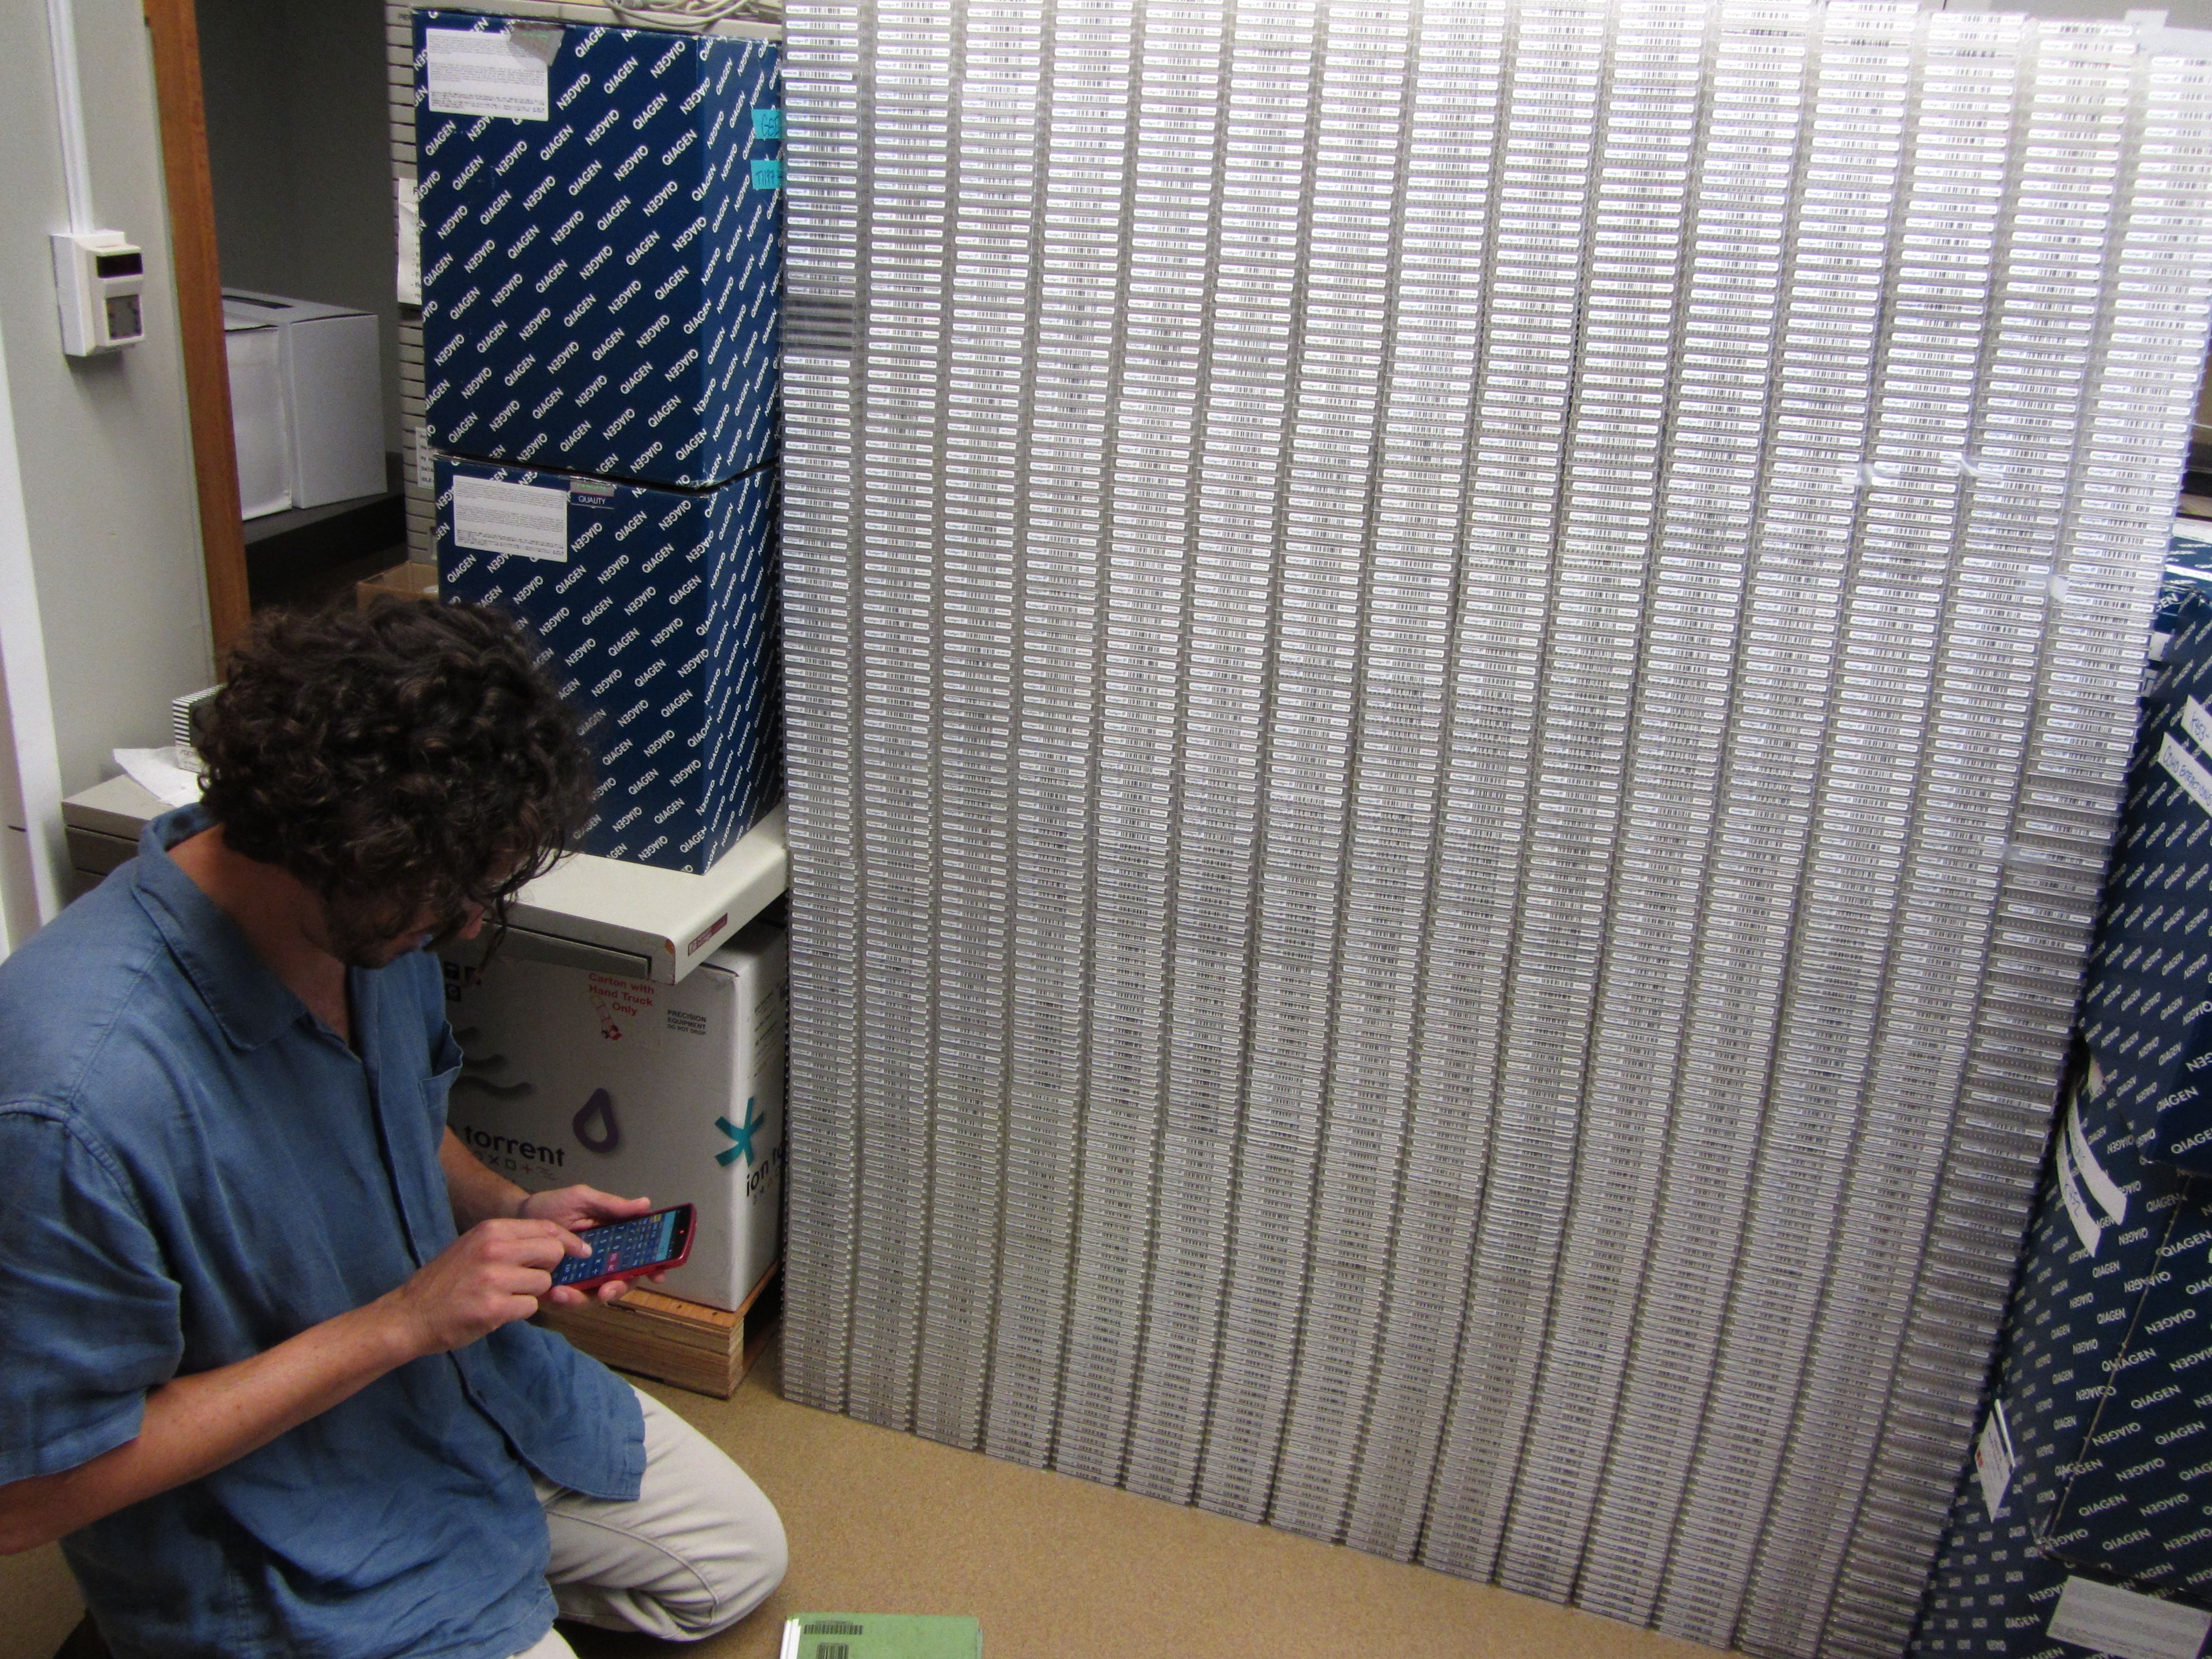
\includegraphics[width=0.75\textwidth]{mhap_figs/AC_calculating_chipwall.jpg}
\end{center}
$\bullet$ However, 96 SNPs are not enough for single parent assignments,\\
$\bullet$ and species ID in juveniles is unreliable
\end{frame}








\begin{frame}{Visual Species ID of juveniles is difficult}
\framesubtitle{Kelp, Gopher, Black-and-yellow indistinguishable at small size}
\begin{columns}
\begin{column}{0.50\textwidth}
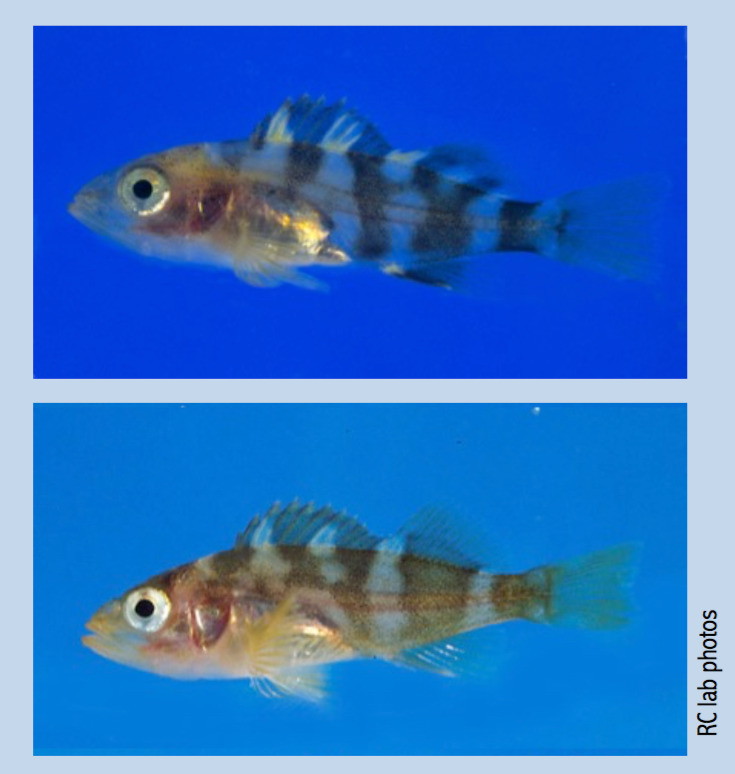
\includegraphics[width=\textwidth]{./mhap_figs/juvie_rockfish.png}
\end{column}
\begin{column}{0.50\textwidth}
\begin{itemize}
\item Up to 40\% of juvenile samples might not be kelp rockfish
\item SNP assays in non-target species tend to be monomorphic, and hence 
useless for any inference.
\item It hurts to contemplate throwing away that much
genotyping effort.
\end{itemize}
\end{column}
\end{columns}
\end{frame}










\begin{frame}{Developing GTseq Amplicons for Rockfish}
\begin{itemize}
\item ddRAD seq on 16 individuals 
\item $\approx 4,000$ genome fragments sequences
\item 200 developed into amplicons, and tested
\item 165 amplicons retained
\item Amplified and sequenced from 240 individuals.
\item Allele/Haplotype frequencies estimated
\begin{itemize}
\item 825 alleles (average of 5 haplotypes per locus)
\end{itemize}

\item Power for Parentage and Full sibling inference computed
\end{itemize}

\end{frame}
















\begin{frame}{Log-likelihood ratio distribution}
\framesubtitle{For Parent-offspring and full-sib pairs vs Unrelated}
\begin{center}
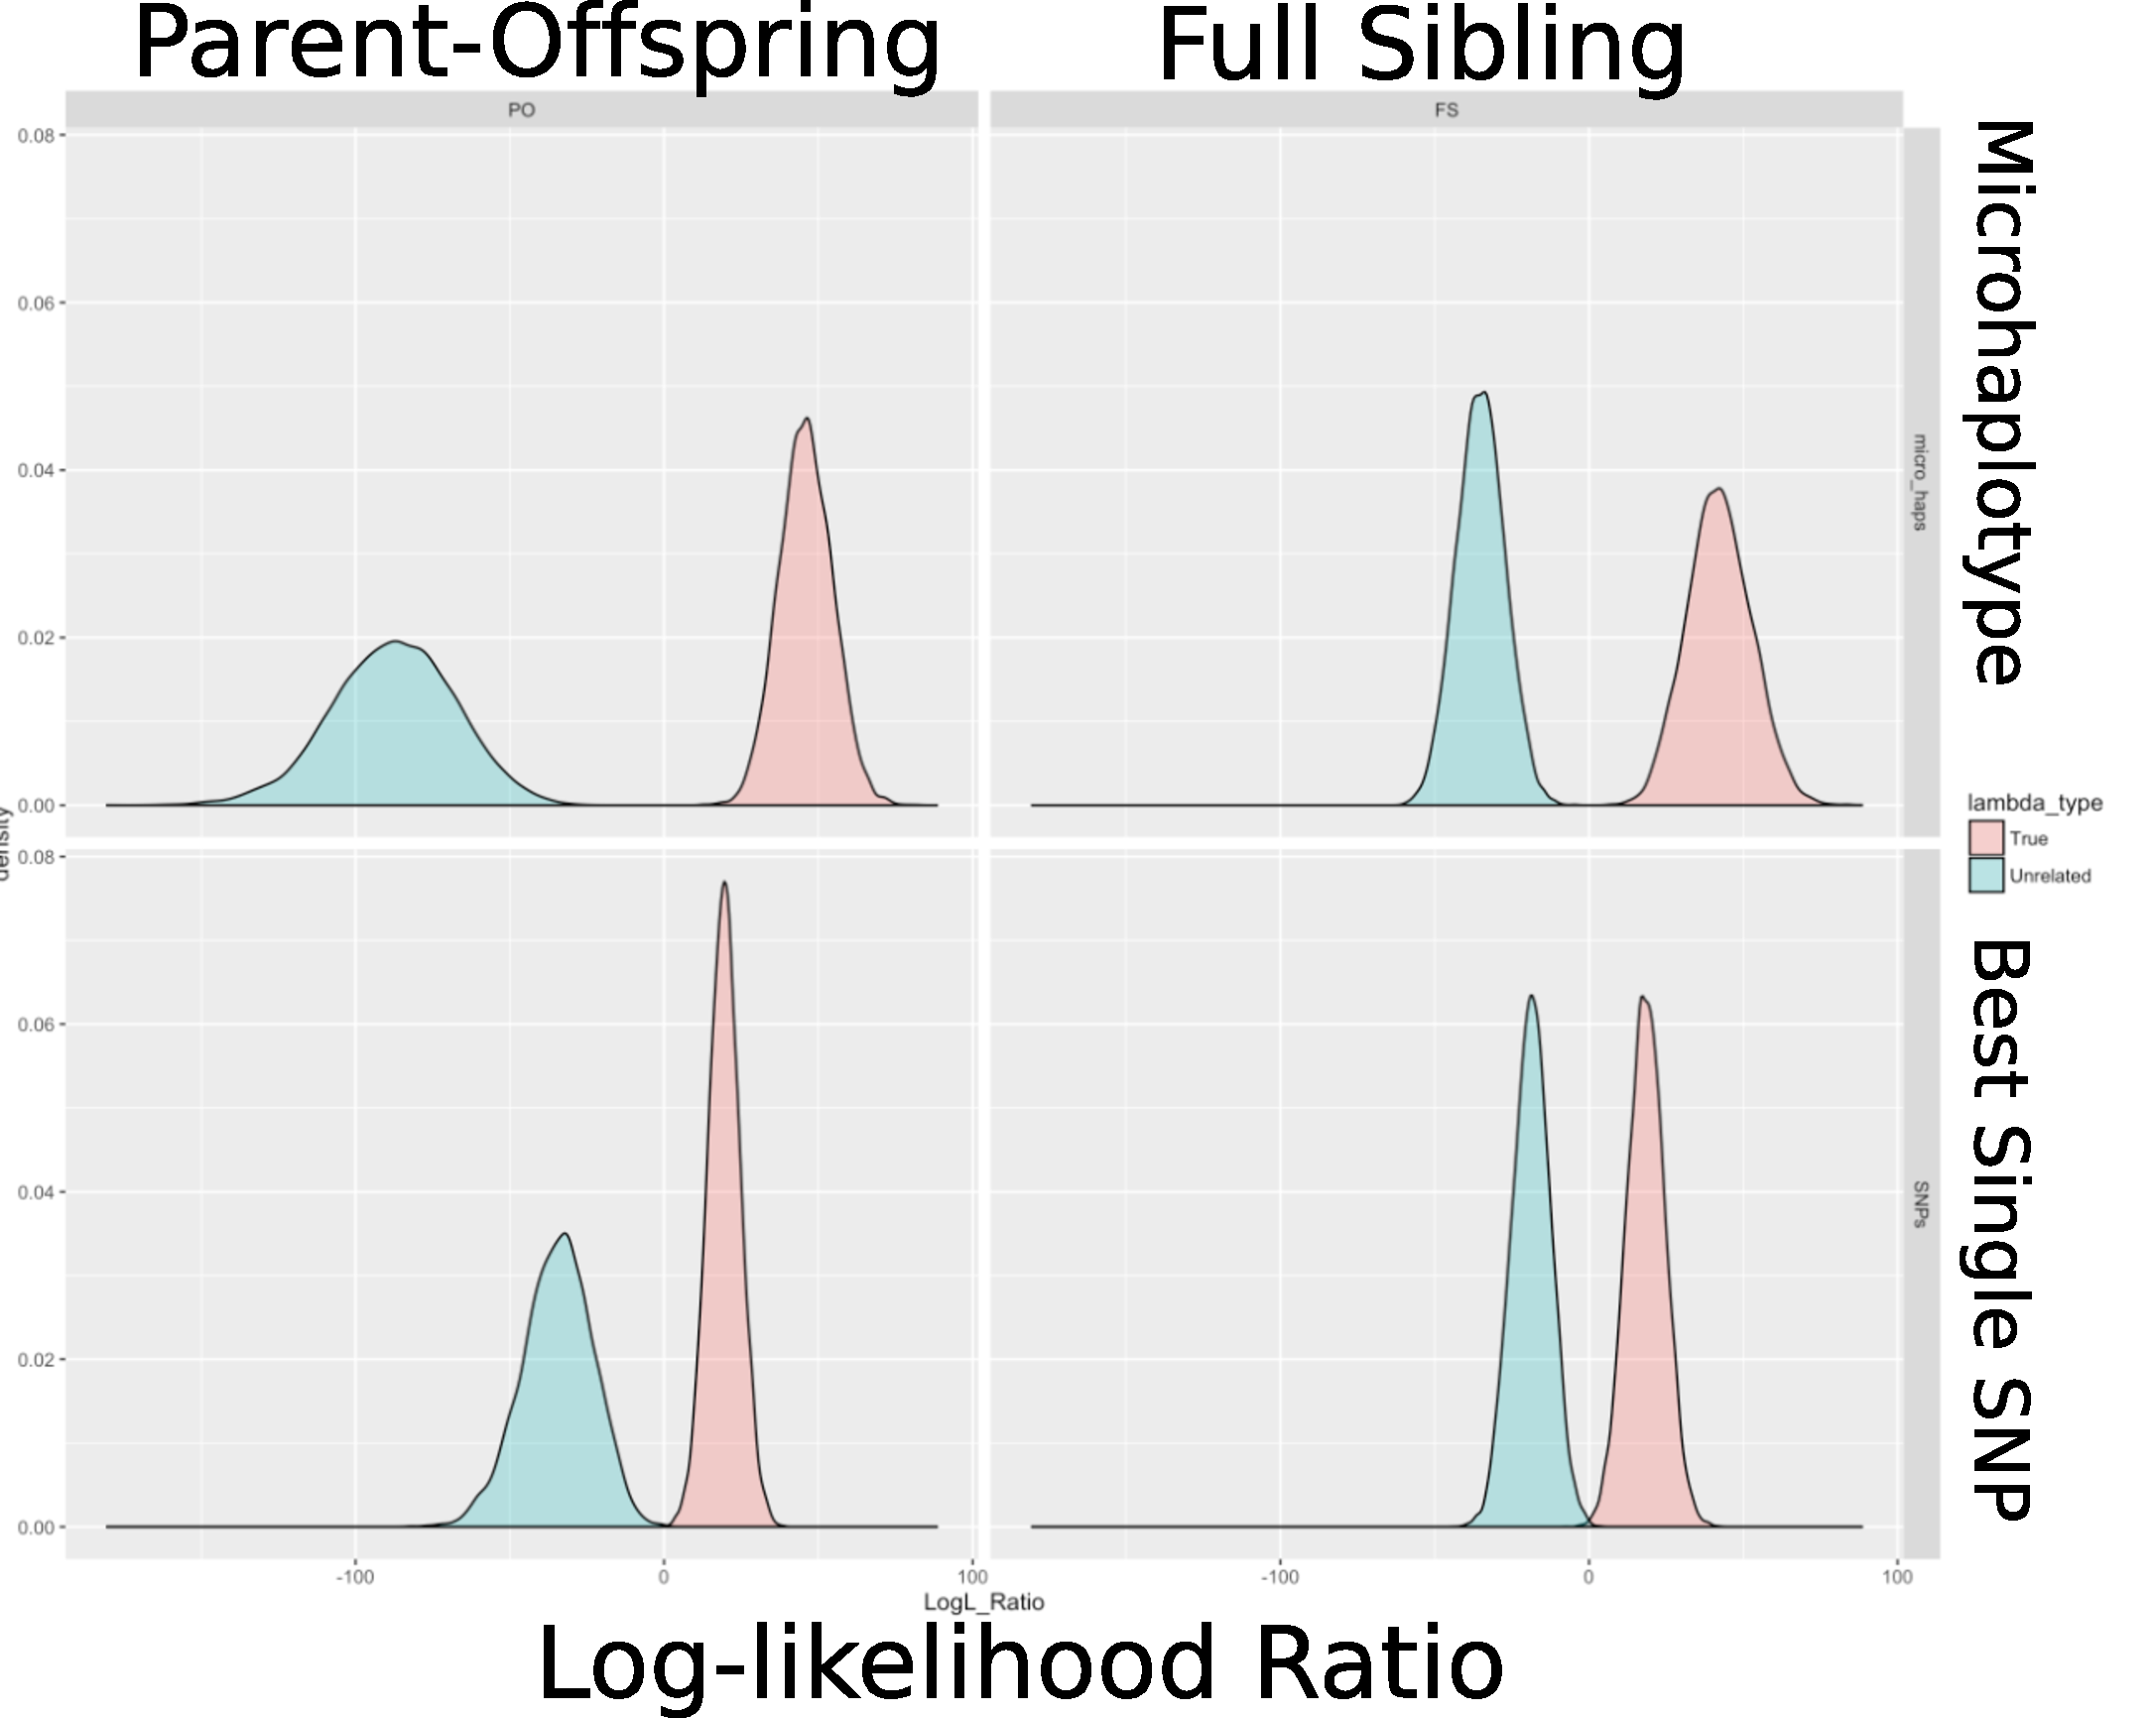
\includegraphics[width = 0.84\textwidth]{mhap_figs/loglrats.pdf}
\end{center}

\end{frame}













\begin{frame}{Log-likelihood ratio distribution}
\framesubtitle{False Positive Rates for Unrelated individuals at False Negative Rate = 1\%}
\begin{center}
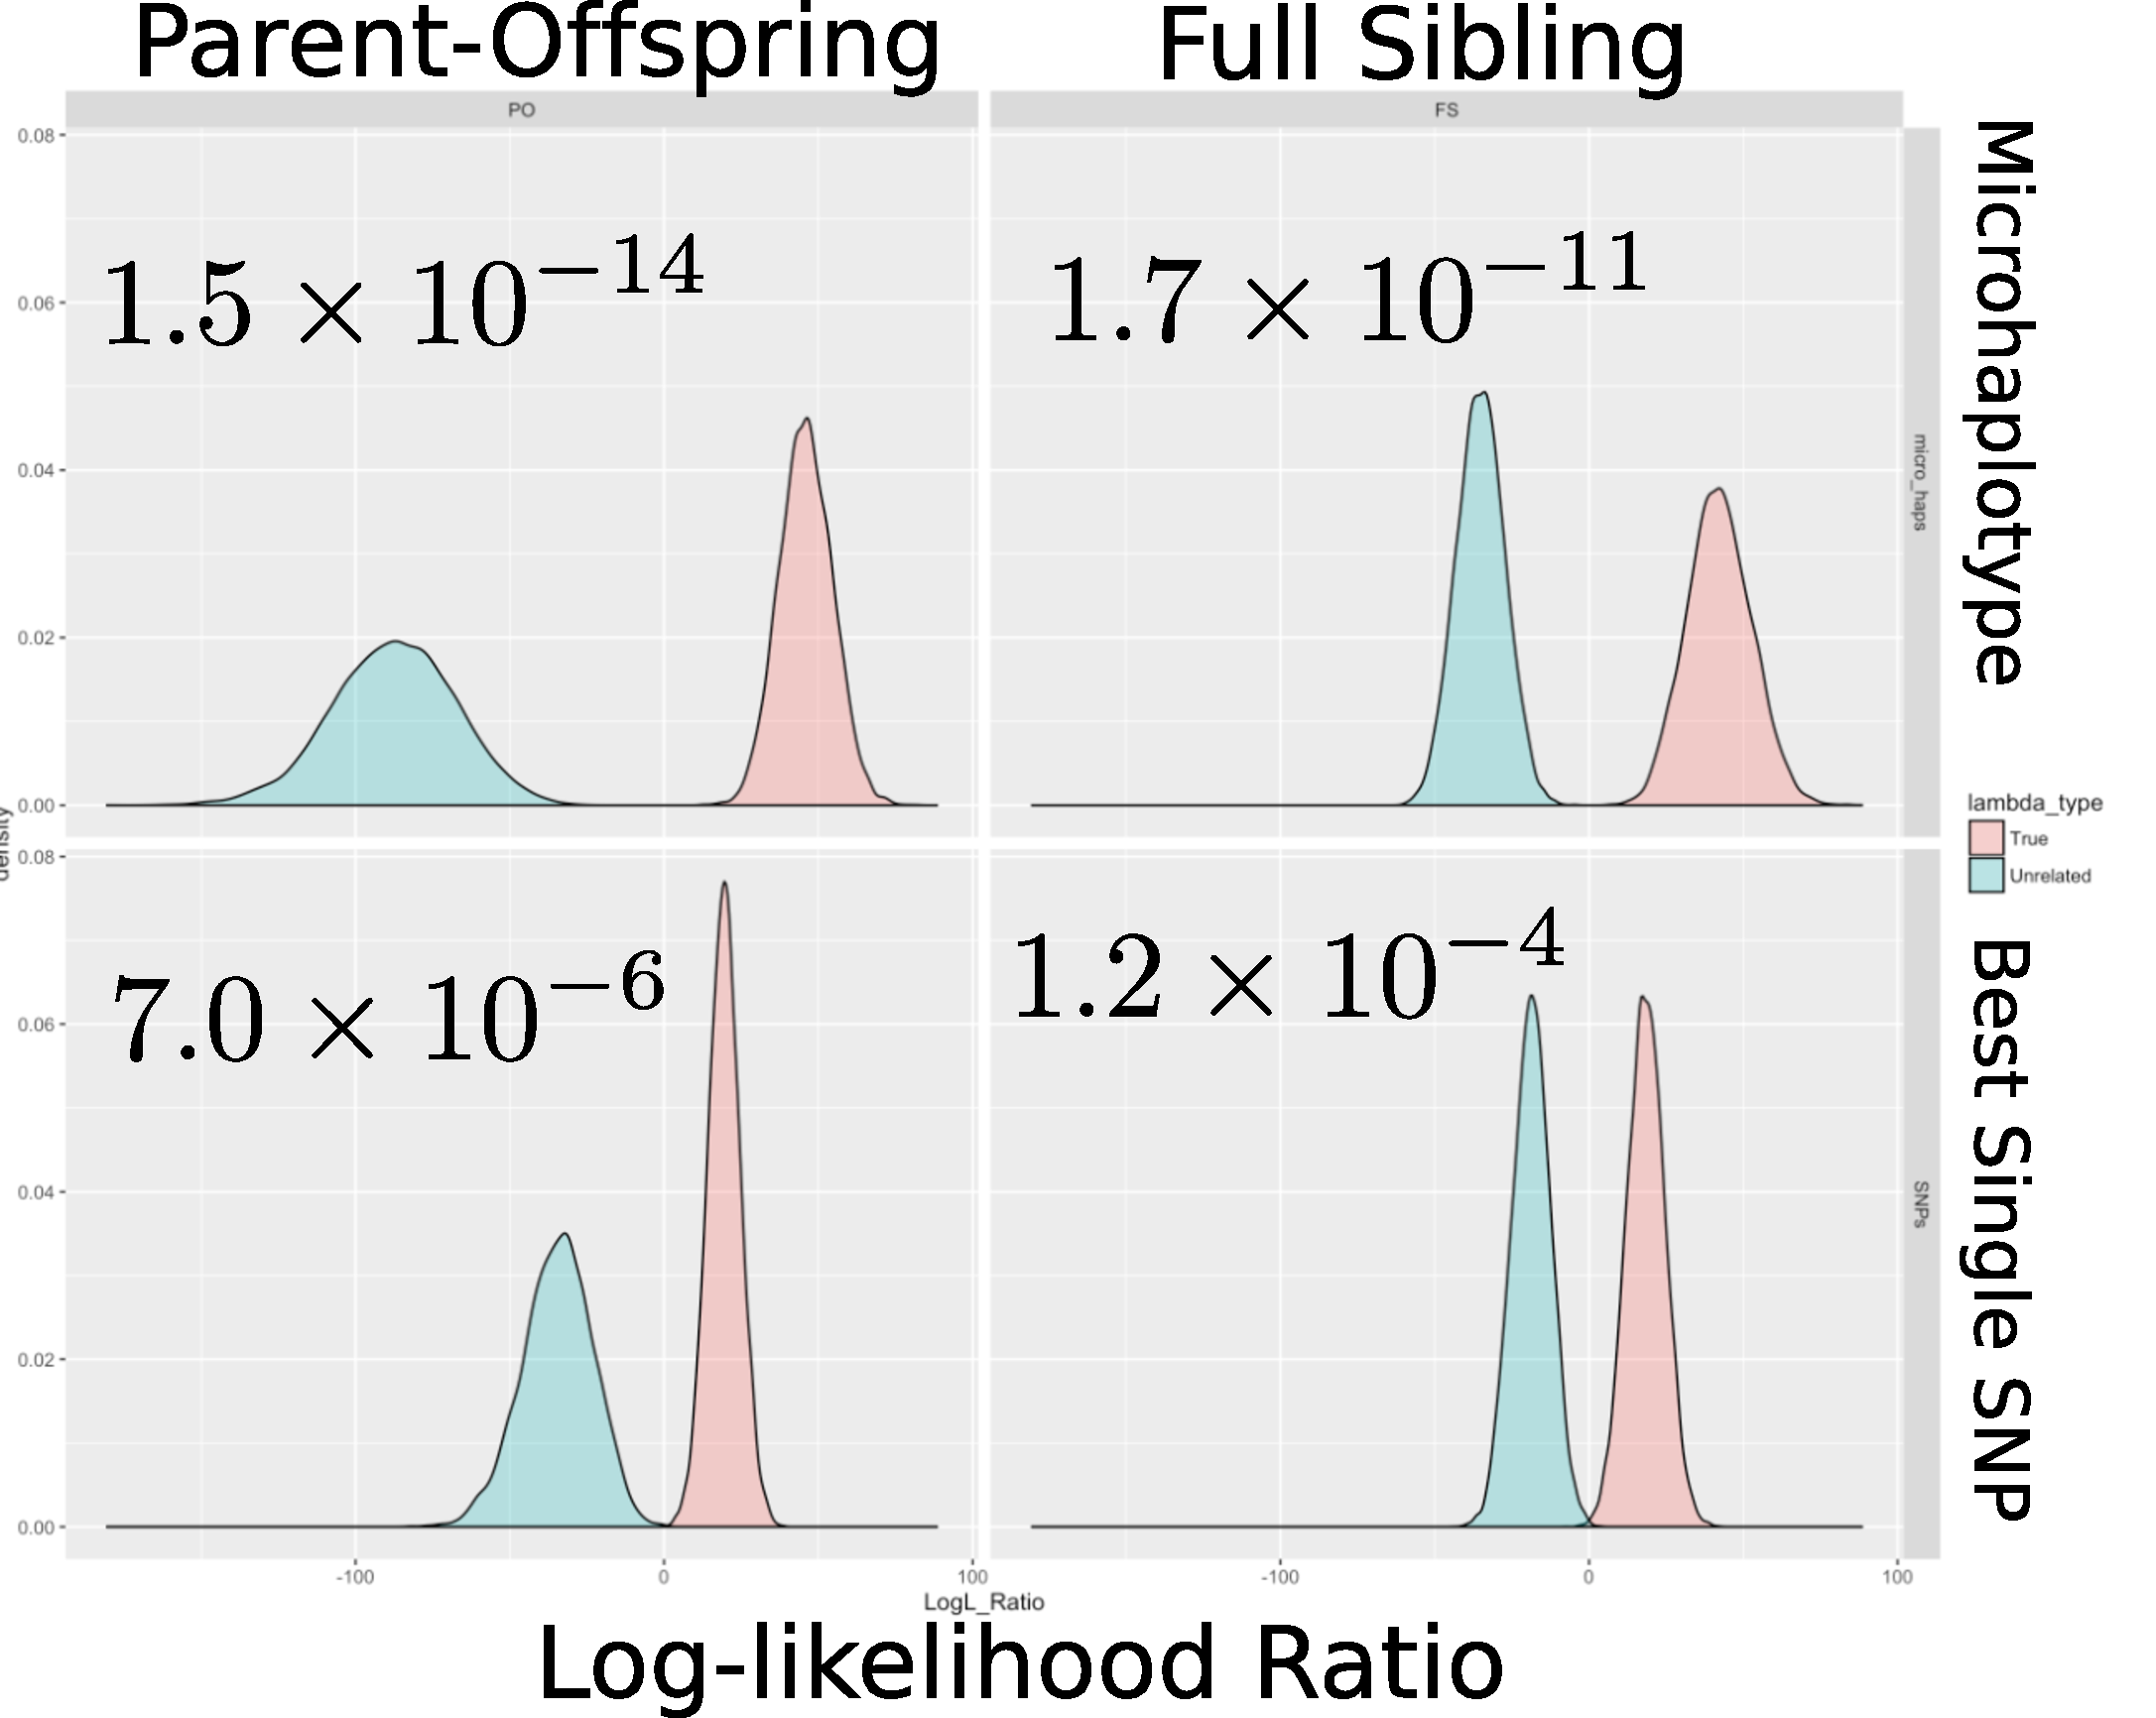
\includegraphics[width = 0.84\textwidth]{mhap_figs/loglrats-FPR.pdf}
\end{center}

\end{frame}












\begin{frame}{Outstanding for Relationship Inference}
\begin{itemize}
\item A false positive rate of $1.5 \times 10^{-14}$ means you could compare 1 million candidate parents to 1 million unrelated candidate offspring and not expect any errors.
\item Using just a single SNP from each locus you would expect 7 errors when comparing 1,000 candidate parents to 1,000 unrelated candidate offspring.
\item Genotyping costs dropping toward $<$\textsterling 5 per sample.
\item Very exciting for ``close-kin mark-recapture''\\
{\em Statistical Science}~31:259--274. (2016)
\end{itemize}
\begin{center}

\includegraphics[width = 0.7\textwidth]{mhap_figs/ckmr-header.png}
\end{center}
\end{frame}









\end{document}





\newlength{\picht}
\setlength{\picht}{3.7ex}
\begin{frame}{The MEGA Team}
\mbox{}\hspace*{-2em}
\begin{tabular}{ll}
\includegraphics[height=\picht]{./images/carlos_garza.jpg}~Dr.~Carlos Garza, {\scriptsize NOAA} &   
\includegraphics[height=\picht]{./images/Vanessa_Apkenas.jpg}~Vanessa Apkenas, {\scriptsize UCSC}\\
%
\includegraphics[height=\picht]{./images/eric_anderson.jpg}~Dr.~Eric C. Anderson, {\scriptsize NOAA} &
~~~~~~~~~Cassie Columbus, {\scriptsize UCSC} \\
%
\includegraphics[height=\picht]{./images/devon_pearse.jpg}~Dr.~Devon Pearse, {\scriptsize NOAA} & 
\includegraphics[height=\picht]{./images/alicia_abadia.jpg}~Alicia Abad\'{i}a-Cardoso, {\scriptsize UCSC} \\
%
\includegraphics[height=\picht]{./images/libby_gilbert.jpg}~Libby~Gilbert-Horvath, {\scriptsize NOAA} &
\includegraphics[height=\picht]{./images/Martha_Arciniega.jpg}~Martha Arciniega, {\scriptsize UCSC} \\
%
\includegraphics[height=\picht]{./images/Eric_Crandall.jpg}~Dr.~Eric Crandall, {\scriptsize UCSC (CSUMB)} &
\includegraphics[height=\picht]{./images/anthony_clemento.jpg}~Anthony Clemento, {\scriptsize UCSC}  \\
%
\includegraphics[height=\picht]{./images/dan_barshis.jpg}~Dr.~Daniel Barshis, {\scriptsize UCSC (9/12)} &
\includegraphics[height=\picht]{./images/hilary_starks.jpg}~Hilary Starks, {\scriptsize UCSC}  \\
~~~~~~~~~Vicky Pritchard  &  ~~~~~~~~~Veronica Mayorga
\end{tabular}
\end{frame}

%\begin{frame}{Outline}
%  \tableofcontents
  % You might wish to add the option [pausesections]
%\end{frame}




\section{Early Years, 2003--2006}
\subsection{Fertile ground}



%%% 	HATCHERY MAP
\begin{frame}{Salmon hatcheries abound}
\begin{columns}
\column{.50\textwidth}
{\centering
\includegraphics[height=6cm]{images/hatcheries.jpg}\\
{\tiny http://www.inforain.org/maparchive/hatcheries.htm}
}
\column{.50\textwidth}
\begin{itemize}
\item Millions of salmon are produced annually in hatcheries.
\item Identifying fishery landings and escapement to hatchery and cohort, one can parameterize salmon ocean forecasting models.
\end{itemize}
\end{columns}
\end{frame}




%% CODED WIRE TAGS
\begin{frame}{Coded Wire Tag Program}
\begin{center}
\mbox{}
\hfill
\includegraphics[height=.33\textwidth]{./images/finger.jpg}
\hfill
\includegraphics[height=.2\textwidth]{./images/cwt.png}
\hfill
\includegraphics[height=.25\textwidth]{./images/pink.png}
\hfill
\mbox{}
\end{center}
\begin{center}
\includegraphics[width=.6\textwidth]{./images/adiposeclip.jpg}
\end{center}
\end{frame}







%% CHALLENGES FACING CWT PROGRAM
\begin{frame}{Challenges Facing the CWT Program Today}
\begin{itemize}
\item Very low tag recovery rates (1.6 per 1,000 in chinook)
\item Tag loss rates are poorly known
\item CWT harvest may be underreported
\item Mass-marking for mark-selective fisheries (THE BIGGIE)
\begin{itemize}
\item Not all Ad-clipped fish have CWT's
\end{itemize}
\end{itemize}

The Pacific Salmon Commission convened an Expert Panel to address these concerns and explore alternatives to / augmentations for the CWT program.
\end{frame}



\subsection{Carlos plants a seed!}
%% FPG SLIDE
\begin{frame}{Parentage Based Tagging (PBT)}
\centering{
\includegraphics[width=.7\textwidth]{./images/genvarpink.jpg}
}
{\small
\begin{itemize}
\item Genotyping all hatchery parents you can create a data base of possible parent pairs and match recovered offspring genotypes against that, assigning offspring to parent pairs (and hence hatchery and cohort).
\item By genotyping two parents, you can effectively tag all their 1,000's of offspring.
\item Also provides scientifically interesting pedigree information.
\end{itemize}
}
\end{frame}


%%% SNP Notation Slide
\begin{frame}{Single Nucleotide Polymorphisms (SNPs)}
\includegraphics[width=.8\textwidth]{images/chromosome.pdf}
{\small
\begin{itemize}
\item  There are usually only two types of bases (letters) found at any SNP.
\item Per-SNP genotyping costs were dropping quickly (for humans) 
\item Can be scored reliably without human intervention
\item Eschewed at the time for inference of relationships 
\end{itemize}
}
\end{frame}




%%% Simple Parentage DAG
%\begin{frame}{Mendelian Inheritance}
%\framesubtitle{The cornerstone of parentage inference}
%\begin{itemize}
%\item Assume two alleles: 0 at freq $q$ and 1 at freq $p$
%\item Every individual inherits one chromosome from its mother and one from its father.
%\end{itemize}
%\includegraphics[height=.23\textheight]{./images/mapa_trio.pdf} 
%\hfill \raisebox{.12\textheight}{$\mathrm{Pr(Trio | Parental)} = q^2\times 2pq \times \frac{1}{2}$ }\hfill \mbox{}

%\mbox{}

%\hrule

%\mbox{}

%\mbox{}

%\includegraphics[height=.23\textheight]{./images/unrel_trio.pdf} 
%\hfill \raisebox{.12\textheight}{$\mathrm{Pr(Trio | Unrelated)} = q^2\times 2pq \times 2pq $}\hfill \mbox{}
%\begin{itemize}
%\item With some extra stuff to account for genotyping error\dots
%\end{itemize}

%\end{frame}

%

%
%%% Log-likelihood ratio statistic
%\begin{frame}{Log-Likelihood Ratio Statistic}
%\framesubtitle{For classifying trios as Parental or Unrelated}
%{\small
%\begin{itemize}
%\item The probability of the genotypes of the trio may be computed for $L$ SNP loci, and under the two different assumptions of ``Parental" or ``Unrelated":
%\end{itemize}
%\begin{eqnarray*}
%P_P = \mathrm{Pr(Trio~|~Parental)}  & = & \prod_{ k=1}^{L}\mathrm{Pr_ k(Trio~|~Parental}) \\
%P_U = \mathrm{Pr(Trio~|~Unrelated)}  & = & \prod_{ k=1}^{L}\mathrm{Pr_ k(Trio~|~Unrelated}) \\
%\end{eqnarray*} 
%The Log-Likelihood Ratio statistic is just the log of the ratio of those two probabilities.  
%\[
%\Lambda(G) = \log\frac{P_P(G)}{P_U(G)}
%\]
%}
%\end{frame}

%

%

%%% Color Distribution
%\begin{frame}
%\begin{center}
%\includegraphics[width=\textwidth]{./images/TriosColor.pdf}
%\end{center}
%{\scriptsize
%\begin{itemize}
%\item False negative rate = Probability of incorrectly classifying a true parental trio as unrelated
%\item False positive rate = Probability of wrongly declaring an unrelated trio as parental
%\end{itemize}
%}
%\end{frame}


\begin{frame}{Importance sampling for power of SNPs}
\framesubtitle{Anderson and Garza (2006) {\em Genetics}}
%\begin{columns}
%\column{.4\textwidth}
%~~~~~~\includegraphics[width=\textwidth]{images/fprs.png}
%\column{.6\textwidth}
\vspace*{-2.2ex}
\begin{center}
\includegraphics[width=.83\textwidth]{images/andgar.png}
\end{center}
\begin{itemize}
\item Exponential decrease of false positive rates with number of SNPs
\item Around 100 SNPs yields FPR of $10^{-13}$
\item Need more power? Add another 20 SNPs
\item Wow! This could work! (At least {\em we} were convinced it could work!)
\end{itemize}
\end{frame}


%\begin{frame}{Quick overview of PBT's methodological development}
%\framesubtitle{With particular emphasis on co-author's roles}
%\vspace*{-1.2ex}
%\begin{itemize}
%\item \mbox{}\includegraphics[height=4ex]{./images/carlos_garza.jpg} {\bf Carlos Garza}: visionary, stalwart PBT developer.
%\item \mbox{}\includegraphics[height=4ex]{./images/eric_anderson.jpg} {\bf Me}: statistician-guy, developed theory (Anderson and Garza 2006, {\em Genetics}) and software ({\sc snppit}) to make PBT possible. Owe huge thanks and acknowledgments to my coathors, and the countless contributors to this project, both within and beyond SWFSC, notably CDFG staff and hatchery staff.
%\item \mbox{}\includegraphics[height=4ex]{./images/anthony_clemento.jpg} {\bf Anthony Clemento}: SNP discovery (95 SNP panel), genotyping, Chinook and FRH pilot study.
%\item \mbox{}\includegraphics[height=4ex]{./images/alicia_abadia.jpg} {\bf Alicia Abad\'{i}a}: SNP discovery (96 SNP panel), genotyping, Steelhead and Russian River pilot study.
%\end{itemize}
%\end{frame}


\subsection{Laying down some roots}
\begin{frame}{Laying down some roots -- I}
\framesubtitle{Developing the SNPs}
{\bf Problem 1}: Only 9 SNPs were known in chinook salmon at the time, and these were biased toward polymorphisms in Alaska:
\begin{center}
\includegraphics[width=.85\textwidth]{images/smithetal.png}
\end{center}
{\bf Solution:} Massive\footnote{Each determined the sequence of 2 to 3 million bases of DNA!!} sequencing efforts by Clemento (chinook), Abad\'{i}a-Cardoso (steelhead), Starks (coho), and Vicky Pritchard (Cutthroat).
\end{frame}

\begin{frame}{}
\begin{columns}
\column{.5\textwidth}
\begin{itemize}
\item Used genomic resources of {\em O.~mykiss} to "amplify" roughly 500 fragments of sequence in each species.
\item Roughly 220 fragments were successfully sequenced.  
\item Yielded about 170 SNPs per spp.~that were good candidates for PBT.
\end{itemize}

\column{.5\textwidth}
\includegraphics[width=.95\textwidth]{images/3730seq.jpg}

\end{columns}

\end{frame}


\begin{frame}{Laying down some roots -- II}
\framesubtitle{Begin collecting spawner samples}
Feather River Hatchery Spring Run Chinook; Warm Springs Hatchery Steelhead; Iron Gate Hatchery Coho

\includegraphics[width=\textwidth]{images/frh.jpg}

\end{frame}



%\begin{frame}{Not everyone shared our enthusiasm}
%\begin{center}
%\includegraphics[height=.8\textheight]{images/garfield.png}
%\end{center}
%\end{frame}


\section{Middle Years, 2006--2010}
\subsection{Our sapling grows up}

\begin{frame}{Advances in genotyping technology}
\begin{center}
\mbox{}\hspace*{-.10\textwidth}
\includegraphics[width=1.16\textwidth]{images/fluidigm.png}
\\
With 96.96 Arrays and only one controller and thermal cycler, \\
can genotype almost 300 fish per day w/96 SNPs!

Cost: $<$\$20/fish (making PBT easily competitive with CWTs)
\end{center}
\end{frame}



\begin{frame}{Fluidigm SNP Genotypes}
\framesubtitle{Very low genotyping error rates. Easily standardized across labs.}
\vspace*{-4.5ex}
\begin{center}
\includegraphics[height=.6\textheight]{images/fluidigm_cartesian.png}~~~~~~~~
\includegraphics[height=.6\textheight]{images/fluidigm_heatmap.png}
\end{center}
\end{frame}


\begin{frame}{Selecting a Panel of 96 SNPs-I}
\framesubtitle{Satisfying tradeoffs between populations}
\begin{columns}
\column{.5\textwidth}
{\scriptsize
\begin{tabular}{lrrr}
FNR:&0.1&0.05&0.01\\ \hline
ButteSp&3.8e-13&2.4e-12&4.9e-11 \\
MillSp&1.3e-13&7.6e-13&1.7e-11 \\
DeerSp&1.4e-13&8.5e-13&1.7e-11 \\
FRHsp&1.0e-13&5.9e-13&1.4e-11 \\
CVFall&1.7e-13&1.0e-12&2.3e-11 \\
UpSacLFall&1.8e-13&1.1e-12&2.3e-11 \\
SacWinter&2.9e-12&1.5e-11&3.0e-10 \\
EelVA&2.9e-12&1.5e-11&3.6e-10 \\
KlamIGH&1.5e-12&8.2e-12&1.8e-10 \\
TrinityH&2.3e-12&1.3e-11&2.8e-10 \\
RogueSp&3.6e-13&2.2e-12&4.8e-11 \\
Chetco&3.0e-13&1.5e-12&4.2e-11 \\
Umpqua&1.2e-13&6.9e-13&1.7e-11 \\
Kalama&2.3e-13&1.4e-12&2.9e-11 \\
Cowlitz&2.7e-13&1.6e-12&4.2e-11 \\
Snake&2.5e-13&1.4e-12&3.0e-11 \\
\end{tabular}
}

\column{.5\textwidth}
Take Home Messages:
\begin{itemize}
\item Single panel of 96 SNPs
\item Sufficient power in most populations
\item From California to Columbia River
\end{itemize}



\end{columns}
\end{frame}




\begin{frame}{Selecting a Panel of 96 SNPs-II}
\framesubtitle{Ensuring they are useful for Genetic Stock Identification (GSI)}
\begin{columns}
\column{.4\textwidth}
\begin{itemize}
\item Identify population of origin of fish
\item \ldots but not cohort
\item Using pre-existing genetic differences between populations
\item Not specific parents
\end{itemize}

\column{.6\textwidth}
\includegraphics[width=\textwidth]{images/mixifishy.png}

\end{columns}
\end{frame}



\begin{frame}{These SNPs are great for GSI}
\includegraphics[width=\textwidth]{images/mix_and_crossval200_for_talk_no_genetics.pdf}
\end{frame}



\begin{frame}{These SNPs are great for GSI}
\includegraphics[width=\textwidth]{images/mix_and_crossval200_for_talk_with_genetics.pdf}
\end{frame}





\begin{frame}{SNPPIT Software}
\framesubtitle{Single Nucleotide Polymorphism Program for Intergenerational Tagging. Funded by the US Section of the Chinook Technical Committee,  Pacific Salmon Commission}
\begin{columns} 
\begin{column}[c]{5cm} 
\includegraphics[width=\textwidth]{images/soft_web.png}
\end{column} 
\begin{column}[c]{5cm} 
%\includegraphics[width=\textwidth]{images/mathy_squash.pdf}
\begin{itemize}
\item Handles very large data sets\ldots quickly!
\item Designed for multiple populations with
	 different allele frequencies 
\item PC and Mac Versions
\end{itemize}
\hrule
\begin{itemize}
\item Input: two-column data
\item Output: kids assigned to parents in descending order of confidence with FDR estimates for each
\end{itemize}
\end{column} 
\end{columns} 
\end{frame}



\begin{frame}{Gratuitous Math Slide}
\begin{columns}
\column{.6\textwidth}
\includegraphics[width=.87\textwidth]{images/tpb.png}
\column{.4\textwidth}
\includegraphics[width=.87\textwidth]{images/sagmb.png}
\end{columns}
\end{frame}








\subsection{Enjoying the shade}

\begin{frame}{Mixed Stock Fisheries for Chinook Salmon}
\begin{itemize}
\item Historically huge fishery for salmon in California ocean. Currently \$100-200M/year. Over \$1B/year in entire Pacific Ocean
\item Mixed fishery: fish from many populations (stocks) comingle in the ocean
\item Some stocks rare and protected, others are abundant and can be harvested
\item Commercial fisheries in California heavily restricted in 2006-2007, closed 1st time ever in 2008-2009: 1st Klamath River \& California Coastal stocks were ``weak'', then the Central Valley stocks\ldots
\end{itemize}
\end{frame}




\begin{frame}{West Coast GSI Collaborative}
\begin{columns}
\column{.5\textwidth}
\begin{itemize}
\small
\item Collaboration between scientists and the commercial salmon fishing fleet
\item Large scale non-retention sampling of fish stratified in time (May-Sep) \& space 
\item Exact GPS coordinates of catch locations and tracklines of all fishing effort
\item 2010 Efforts, May--Sept:
\begin{itemize}
\item 2,683 boat days
\item $\approx$5,500 samples in CA
\item $\approx$5,000 genetic IDs
\item validated with 1,300 physical tags-99\% accuracy
\end{itemize}
\end{itemize}
\column{.5\textwidth}
\includegraphics[height=.85\textheight]{images/wcgsi.pdf}
\end{columns}
\end{frame}



\begin{frame}{Clear Structure in SF Management Zone - 2010}
\begin{columns}
\column{.5\textwidth}
\begin{itemize}
\small
\item Red=Klamath, Green=CA Coastal (Threatened), Blue=Central Valley Fall
\item Significant aggregation apparent by stock
\item Suggests management could profitably be made more precise
\end{itemize}
\column{.5\textwidth}
\includegraphics[height=.85\textheight]{images/sfzone.png}
\end{columns}
\end{frame}







\section{Today and Beyond, 2011--}
\subsection{Lovely blossoms}
\begin{frame}{PBT Pilot Project with FRH Spring Chinook}
\framesubtitle{Anthony Clemento's PhD Dissertation Work}
\begin{columns}
\column{.6\textwidth}
\begin{itemize}
\item Spring-run sampling and genotyping
\begin{itemize}
\item 2006:  1150 [192] = 69\%
\item 2007:  1422 [168] = 78\%
\item 2008:  1537 [431] = 51\%
\item 2009:  1362 [63]
\item 2010:  1963 [222]
\end{itemize}
\item Assigning 2010 broodstock to their potential parents in '06--'08
\item $\approx$1.2 Billion trios
\end{itemize}
\column{.4\textwidth}
\includegraphics[width=.87\textwidth]{images/frh_sign.png}
\end{columns}
\end{frame}






\begin{frame}{About those missing genotypes\ldots}
\framesubtitle{Typically result from injudicious sampling of tissues from ``swimming carcasses''}
{\centering
\includegraphics[width=.85\textwidth]{images/fungus_fish.jpg}
}
\end{frame}







\begin{frame}{FRH Spring Chinook Offspring Assigned to Parents}

\vspace*{-2.7ex}
\begin{center}
\includegraphics[width=\textwidth]{./images/fdrs_all_info.pdf}
\end{center}
1234 out of 1741 fish assigned to parents, at an estimated\\
FDR of 1/200	
\end{frame}




\begin{frame}{FRH Spring Chinook 2009 ``Decoy'' Parents Included}

{\centering
\includegraphics[width=\textwidth]{./images/fdrs_incl_2009.pdf}
}	
$\approx$835,000 parent pairs from 2009 = 60\% of all parent pairs\\
~~~And none are incorrectly identified as parents {\tiny (FDR~is~conservative)}
\end{frame}






\begin{frame}{PBT on mixed-stock, ocean-fishery samples}
\begin{description}
\item[1,806] Chinook port-sampled by CDFG from CA commerical and sport fisheries  
\item[968] of these carried CWTs to give them stock of origin
\item[56] of these CWTs were reported to be from FRH spring run, which is tagged at a rate of 100\%.
\item[41] of these were identified by PBT using our FRH samples.
\end{description}
Note: given age distribution and our sampling fractions, we expect to assign parentage to 44.3 out of 56 fish from FRH Spring.  41 is not significantly different than 44.3 (binomial distribution).  Implies {\em false negative rate} is near 0.  
\end{frame}








\begin{frame}{Evaluating CWT accuracy with PBT}
We can use PBT to assess how accurate the CWTs are for FRH Spring:
\begin{description}
\item[1806] fish genotyped and compared to FRH Spring broodstock
\item[51] of these have parents in FRH Spring (FROM PBT)
\item[41] of these 51 have CWTs indicating FRH Spring
\item[8] of these 51 were sampled by CDFG, but they failed to recover the CWTs from the fish.
\item[2] of these 51 had CWTs that were read to be from {\em i}\/) Coleman Nat.\ FH Late Fall, and {\em ii}\/) Feather River Fall. 
\end{description}
Wow!
\begin{itemize}
\item 8/51 $\approx$ 16\% CWT loss / failure-to-recover rate! 
\item 2/43 $\approx$ 5\% CWT misreading rate!
\end{itemize}
\end{frame}



%\begin{frame}{Estimated FDRs from Ocean Fishery}
%\includegraphics[width=\textwidth]{images/cdfg_fdrs1.pdf}
%\end{frame}

%

%\begin{frame}{Estimated FDRs from Ocean Fishery}
%\includegraphics[width=\textwidth]{images/cdfg_fdrs2.pdf}
%\end{frame}



\subsection{Tasty fruit}


\begin{frame}{PBT in Steelhead {\em Oncorhynchus mykiss}}
\framesubtitle{Alicia Abad\'ia-Cardoso's PhD Dissertation Work}
\includegraphics[width=\textwidth]{images/steelies.png}
\end{frame}




\begin{frame}{Russian River Steelhead Hatcheries}
\begin{columns}
\column{.5\textwidth}
\begin{itemize}
\item WSH: Warm Springs Hatchery
\item CVFF: Coyote Valley Fish Facility
\item Hatchery and wild fish are part of the Threatened Central California Coastal DPS of {\em O. mykiss}
\end{itemize}
\column{.5\textwidth}
\includegraphics[height=.84\textheight]{images/wsh_map.png}
\end{columns}
\end{frame}



\begin{frame}{PBT Sampling and Results}
\framesubtitle{PBT shatters previously held misconceptions at WSH and CVFF}
\vspace*{-1.1ex}
\begin{center}
\includegraphics[width=.8\textwidth]{images/wsh_samp.png}
\\
\mbox{}
\\
\includegraphics[width=.9\textwidth]{images/russ_riv_tab.png}
\end{center}
\end{frame}





\begin{frame}{Estimating Heritability of Spawn-Timing}
\framesubtitle{Just one example of what is possible with pedigree data}
\begin{center}
\includegraphics[width=.9\textwidth]{images/spawn_timing.png}
\end{center}
\end{frame}


\begin{frame}{Other uses of pedigree data from PBT}
\framesubtitle{These applications not typically accessible with CWTs}
\begin{itemize}
\item Variance in family size
\item Quantitative genetic studies of phenotype
\item Map genes for phenotypic traits to locations in the genome
\item Evaluate hatchery practices on marine survival
\item Estimate straying and reproductive success of strays
\item Hatchery domestication studies
\end{itemize}
\end{frame}






\begin{frame}{Summary}
\vspace*{-1ex}
\begin{itemize}
\item Time is ripe to find a viable alternative to CWTs
\item With theoretical reasons to believe PBT would excel we:
	\begin{itemize}
	\item Developed the markers and software necessary
	\item Launched several pilot projects
	\end{itemize}
\item The SNP markers perform well for GSI in CA and have been informative to management in that capacity
\item The pilot projects have demonstrated that
\begin{itemize}
\item PBT works {\em in practice} too!
\item CWT error rates higher than previously appreciated
\item PBT yields valuable biological information not feasibly obtainable from CWTs
\end{itemize}
\item Cost of PBT competitive with CWTs:  For FRH Spr:\\
{\centering $10^6$ juveniles $\times$ \$0.08 = \$80,000/year for wire alone!\\
{\em versus}\\
1,200 broodstock $\times$ \$20/genotype = \$24,000/year for PBT tagging.
} 
\end{itemize}

\end{frame}




\subsection{Large scale production}


\begin{frame}{Full scale production}
\framesubtitle{People have noticed, and PBT is going mainstream}
\begin{itemize}
\item We have buy-in from most hatchery managers in California
\begin{itemize}
\item All non-fall Chinook hatchery programs in California + Feather River Fall and Trinity Hatchery Fall Chinook
\item All the steelhead hatchery programs in California 
\end{itemize}
\item IDFG, early adopters.  Have combined our SNPs with those developed by CRITFC to assess PBT for Snake River Steelhead
\begin{itemize}
\item Using SWFSC software (for both PBT and GSI)
\item Are eager to switch 100\% to PBT
\end{itemize}
\item Most other state {\em genetics} labs are ``on board'' (ADFG, WDFW, etc.)
\item Pacific Salmon Commission and Bonneville Power Administration sponsoring efforts to develop standardized PBT panels, and 
assess feasibility of adopting PBT (Hankin)
\end{itemize}
\end{frame}





\begin{frame}{SWFSC's role moving forward}
\framesubtitle{On both the international and the state scale}
\begin{itemize}
\item SNP panel standardization
\item SQL data base construction
\item New software development
\item  Data transparency and accessibility
\item In CA specifically, ``Complete Life Cycle Monitoring'' with PBT 

\end{itemize}
\end{frame}



\begin{frame}{Acknowledgments}
\framesubtitle{Collaborative effort, sampling, funding, and support from:}
\begin{itemize}
\item {\bf Funding:} Pacific Salmon Commission, US Chinook Technical Committee
\item {\bf Hatchery Staff:} Feather River Hatchery, Warm Springs Hatchery,  Coyote Valley Fish Facility, Iron Gate Hatchery
\item {\bf California Salmon Council:} David Goldenberg, Jim Anderson, Sarah Bates, and many, many fisherman
\item {\bf CDFG, IDFG, WDFW, ADFG, ODFW, CRITFC, USFWS, PSMFC, US-ACE, NWFSC, AFSC, CALFED, OSU, UC}
\item {\bf NMFS/SWFSC Leadership} 
\end{itemize}
\end{frame}



%\bibliography{anderson}
%\bibliographystyle{mychicago}



\end{document}
